\documentclass[doc, a4paper]{apa7}

\usepackage{lipsum}

\usepackage[american]{babel}

\usepackage{minted}
\usepackage{hyperref}
\usepackage{amsmath} 
\usepackage{caption} 
\captionsetup[table]{skip=10pt}
\usepackage{csquotes}
%\usepackage[style=apa,sortcites=true,sorting=nyt,backend=biber]{biblatex}
\usepackage[natbibapa]{apacite}
% the bibliography prints both urls and dois. This may be a solution, but I get some errors: 
% https://tex.stackexchange.com/questions/195512/linebreak-in-url

%\DeclareLanguageMapping{american}{american-apa}
%\addbibresource{bibliography.bib}

\title{Can we utilize Large Language Models (LLMs) to generate useful linguistic corpora? A case study of the word frequency effect in young German readers}
\shorttitle{LLMs for generating linguistic corpora}

\authorsnames[1,2,3,2]{Job Schepens, Hanna Woloszyn, Nicole Marx, Benjamin Gagl}
\authorsaffiliations{{Institute for Linguistics, University of Cologne}, {Self learning systems Lab, University of Cologne},{Mercator Institute, University of Cologne}}

\leftheader{Schepens, Woloszyn, Marx, Gagl}

\abstract{Is a word frequency measure based on a large body of text generated by large language models (LLM) appropriate to model the frequency effect in reading? Here, we created a corpus based on texts generated by an LLM (GPT 3.5) to measure word frequency (i.e., how often a word occurs). We prompted the LLM to write book summaries for young German-speaking readers. The generated texts had a lower lexical richness than the German children's books they summarized. We used reading performance data from German children (i.e., reaction times in a lexical decision task) to investigate the effect of LLM word frequency on visual word recognition. We found that LLM word frequency explained more variance in reading performance from Grades 1-4 when compared to a word frequency measure based on the original children's books (Experiment 1) and also when compared to a word frequency measure based on adult-directed LLM text (Experiment 2). We conclude that LLM corpora are less lexically rich while approximating children's lexical processing well. We discuss the potential of this approach, considering the inevitable risks of using LLMs that lack openness, are highly complex, and need a large amount of resources.}

\keywords{Large language models, linguistic corpus, word frequency effect, lexical decision task}

\authornote{
    \addORCIDlink{Job Schepens}{0000-0003-1271-2526}
    \addORCIDlink{Nicole Marx}{0000-0002-7027-0618}
    \addORCIDlink{Benjamin Gagl}{0000-0002-2339-6293}

    We deeply thank Elen le Foil for their detailed comments and feedback, which greatly improved our work. 

    Correspondence concerning this article should be addressed to Job Schepens, Institute for Linguistics, University of Cologne Albertus-Magnus-Platz, 50923 Köln, Germany. E-mail: job.schepens@uni-koeln.de}

\begin{document}
\maketitle

Large Language Models (LLMs) have, in recent history, improved quickly so that they now allow meaningful interactions between humans and computers across many languages \citep{chang_when_2023, lai_chatgpt_2023} and various contexts, despite their vastly non-human-like nature \citep{min_recent_2021, singhal_large_2023, kasneci_chatgpt_2023}. LLMs have been used in psycholinguistics to generate predictors that describe linguistic stimuli \citep{trott_can_2024}. For example, LLMs have been successful by explaining more variance in eye-movement behavior in the estimation of word predictability out of the sentence context \citep{hofmann_language_2022, chandra_synthetic_2023, heilbron_prediction_2021}, a promising test case since the training of LLMs is also based on optimizing the next-word predictability \citep{tay2022efficienttransformerssurvey}.  Similarly, the occurrence of words in a language, as measured by word frequency (i.e., how often words occur), might be inherent to LLMs. However, word frequency measurement would need an entirely different corpus-generating approach than next-word prediction.

To explore the potential of LLMs to generate text corpora to measure psycholinguistics word characteristics, we here started with measuring word frequency. Word frequency is central to consider in word recognition and reading studies as it has a large effect on adult and child reading performance \cite{brysbaert_impact_2016,brysbaert_word_2018,gregorova_access_2023,schroter_developmental_2017, kliegl_length_2004,hawelka_dual-route_2010} so that psycholinguists cannot ignore it. The frequency of a word is typically measured based on linguistic corpora by counting the number of occurrences of a word in that corpus (e.g., see \cite{brysbaert_word_2011,baayen_celex_1993,schroeder_childlex_2015,heister_dlexdb_2011}). Thus, each new corpus created could come up with a more appropriate word frequency estimate, describing the variance in word recognition tasks better than other existing measures \cite{brysbaert_word_2011}. Here, we investigate whether one can use an LLM corpus to extract a word frequency measure that has the potential to better describe the variance in word recognition performance. 

We start this exploration for beginning German readers, as we expect smaller corpora for this group, generation should be efficient. Also, specifically for this group, two evaluation datasets are already present: (i) The childLex provides a high-quality corpus of 500 books written for children \citep{schroeder_childlex_2015} from which the word frequency measures are available. This dataset allows the direct comparison of LLM-generated corpora with existing book-based corpora using measures like lexical richness and word frequency. (ii) The DeveL \citep{schroter_developmental_2017} provides reading performance data for a large set of words based on reaction times in a lexical decision task. Here, we can compare existing and LLM-based word frequency measures to investigate which measure explains more variance in reading performance. The goal of these evaluations is to test if the integration of LLM corpora into psycholinguistic research is reasonable, potentially identifying a way of using LLM corpora for estimating specific word frequency measures for selected groups (in our case, German school children) to implement more targeted investigations without sufficient psycholinguistic resources.

The effect of word frequency on reading performance is considered substantial and robust \citep{brysbaert_impact_2016, brysbaert_word_2018} across groups \citep[e.g.,][]{hawelka_dual-route_2010} and modalities \citep[e.g.,][]{gregorova_access_2023}. The word frequency effect describes that words that often occur (i.e., high-frequency words) are recognized faster and more accurately compared to less common words \citep[i.e., low-frequency words; ][]{adelman_contextual_2006, baayen_demythologizing_2010, brysbaert_impact_2016, gregorova_access_2023, hallin_effects_2018, lieven_input_2010, mcdonald_rethinking_2001, stokes_neighborhood_2010}. To estimate word frequency accurately, the choice of the underlying corpus is highly relevant. Previous studies have collected large numbers of books and newspapers and combined those into corpora for measuring word frequency \citep[e.g.,][]{baayen_celex_1993, heister_dlexdb_2011}. The use and validity of frequency measures depend on the source of the text. Brysbaert and colleagues \citep{brysbaert_word_2011, brysbaert_word_2018} have shown that word frequency statistics based on television and movie subtitles result in more explained variance in word processing difficulty performance measures such as lexical decision times \citep[see also][]{chilson_films_2024}. The critical comparison here is based on model comparisons utilizing reading performance data; i.e., a regression model involving subtitle-based word frequency measures had a higher model fit than a book-based word frequency measure \citep[see, e.g.,][]{brysbaert_word_2011}. Thus, the corpus used to derive word frequency significantly influences the amount of variance that word frequency can explain \citep{ferrand_french_2010, keuleers_subtlex-nl_2010, van_heuven_subtlex-uk_2014}, even when carefully controlling for other essential word characteristics such as orthographic similarity to other words, age in which a word is typically acquired, and word length \citep{graf_faktorenanalyse_2005}. 

Only a few large linguistic corpora for child-related word frequency exist. These are typically based on children's books or subtitles for children's movies \citep{schroeder_childlex_2015, tellings_basilex_2014, van_heuven_subtlex-uk_2014, Korochkina_2024}. Constructing a corpus of texts targeted explicitly at children is challenging for several reasons. The number of materials directed explicitly for children is necessarily smaller than the adult resources. Access to a wide range of children's literature and other resources can be limited due to, e.g., questionable validity or even availability of listed or estimated target age range. Estimating target age can be problematic, as not all material explicitly indicates a target age group. Finally, there are even fewer resources of children-generated texts \citep[see, e.g.,][]{laarmann-quante_litkey_2019}. Together, such factors result in a limited and possibly biased set of language materials, which is expected to have implications for studies using word frequency measures. 

Previous studies thus show that text type is important for studying the effects of word frequency on reading performance. Adding word frequency measures based on LLM text to the comparison may shed light on the usefulness of LLMs in psycholinguistic research. Our primary objective is to evaluate a measure of word frequency derived from LLM text. We focus on young German readers for two reasons: (i) Existing children's written text corpora and children's word knowledge are smaller than adults. Thus, the generation of an LLM corpus may be more manageable for kids than for adults. (ii) The psycholinguistic resources available for German beginning readers are optimal for systematically comparing the LLM corpus with a classical book-based corpus \citep[childLex;][]{schroeder_childlex_2015}. First, we generate a corpus by choosing prompts that try to reproduce the original corpus based on German children's books by mentioning the titles of the books included in childLex. Then, we directly compare the frequency of all words from both corpora. Finally, we use a large reading performance dataset \citep[DeveL;][]{schroter_developmental_2017} to evaluate the LLM word frequency measures based on reading performance, similar to recent comparisons for evaluating previously developed word frequency measures \citep[e.g.,][]{brysbaert_word_2011, brysbaert_word_2018}. Similar to other studies on word frequency effects, we also decided to use lexical decision performance \citep[i.e., an often-used classical task, that offers a window into understanding word recognition in children;][]{davies_reading_2017, monster_word_2022, van_den_boer_lexical_2012}. Furthermore, recent evidence also suggests that a brain region typically associated with efficient reading \citep{dehaene_unique_2011} is active when performing lexical categorization \citep[i.e., the process underlying lexical decisions;][]{gagl_lexical_2022}) and lexical categorization training can increase reading skill \citep{gagl_investigating_2023}.


\subsection*{Strengths and Weaknesses of using LLMs for Psycholinguistic Research}

LLMs are computational models with a considerable amount of trainable parameters - in the case of ChatGPT-3, 175 billion \citep{brown_language_2020}. This makes the inner workings opaque but potent for learning language-related tasks like next-word or next-sentence prediction with high accuracy \citep[e.g.,][]{devlin2019bertpretrainingdeepbidirectional}. LLMs make use of architectural principles such as transformers and attention heads \cite[\cite{vaswani_attention_2017}; See also][for an introduction]{hussain_tutorial_2024}). To be able to produce comprehensible output text, LLMs need to be trained on a vast set of data \citep{bender_dangers_2021}. From these aspects of LLMs, a number of problems become evident. 

Little is known about the minimal training data requirements \citep{hosseini_artificial_2022}. Current datasets are considered not "developmentally realistic" when compared to the input of humans. Also, the required amounts of computing resources and training data can make it technically challenging to apply interventions or change aspects of the architecture or training procedure, so they are typically fine-tuned using reinforcement learning with human feedback (RLHF) to generate output that aligns with desired outcomes \citep[see][for how to remove troubling model outputs]{ouyang_training_2022}. Given the unavoidable bias in the training data and process, the output of LLMs is biased in favor of Western culture \citep{atari_which_2023}. Furthermore, for most monetized LLMs, no precise numbers on the characteristics are available as they lack transparency \citep{liesenfeld_opening_2023, frank_openly_2023}. The lack of transparency and the enormous effort in training these models make reproducing the model frameworks impossible (as we show in the comparison of Experiments 1 and 2), questioning what kind of LLMs should be and not be used in research or as research objects \citep{bender_dangers_2021, liesenfeld_opening_2023}. 

Despite the weaknesses, LLMs can have seen more words (and possibly languages) than any human. Their training is focused on the context in which words are presented (i.e., next-word prediction). Extensive training data in combination with the next-word-prediction training task may be a strength for estimating word frequency compared to traditional measures since estimating the probability of words is part of how LLMs are trained. Furthermore, estimating word frequency from LLM text can be considered as near transfer (word frequency and probability are closely related). Near transfer arguably is less noisy compared to far transfer, e.g., studying language comprehension \citep{Dentella_2024}, which would be less closely related to the LLM training procedures. In addition, how often a word is present in LLM text has a good chance of being informative when planning to measure its frequency in a language. Finally, the output of LLMs is generally flexible. It depends on the model prompt and a set of parameters (e.g., the temperature parameter: Higher values lead to greater lexical diversity in the generated text, similar to exploration in humans \citep{momennejad_evaluating_2023}). 


%One could argue that human minds, i.e., the origin of books or subtitles, is also a black box that psychology and neuroscience have not yet fully explained. Thus, generating word frequency statistics from one or the other black box could be seen as equally troubling.

Are LLMs usable as models for research on language processing? So far, LLMs have been used to expose necessary conditions and qualities of the learning environments for human language acquisition \citep{warstadt_findings_2023, trott_large_2023}, predict human brain responses to language \citep{tuckute_driving_2024}, can be used for the estimation of word predictability out of the sentence context \citep{hofmann_language_2022, chandra_synthetic_2023, heilbron_prediction_2021}, and explain N400 effects \citep{michaelov_strong_2024}, but are still inaccurate when language needs to be comprehended \citep{Dentella_2024}. Such efforts indicate the importance of human benchmarks, which are necessary to evaluate how LLM capacities are human-like. Using LLMs for studying human cognition is, however, relatively new. LLMs deviate from human behavior in significant ways \citep{mahowald_dissociating_2024}, including the fact that LLM optimization is very different from the pressures that shape human performance \citep{mccoy_embers_2023}. Concerning (child) reading research, the vast training data and training procedure may enable LLMs to represent various linguistic contexts and reflect children's exposure to different words in ways relevant to word frequency measurement. We test the latter aspect here. 


\subsection*{Present study}

Here, we want to explore, in two experiments, if and how LLMs can produce corpora for measuring word frequency appropriate for the approximation of the lexicon of young German readers. ChildLex \cite{schroeder_childlex_2015}, our reference corpus, is based on children's books. In Experiment 1, we generate one corpus that is modeled after ChildLex \cite{schroeder_childlex_2015}. To implement this, we prompt the model for child-directed summaries of the books included in the original corpus. In Experiment 2, we generate four more corpora, in which we systematically vary the prompt (i.e., child vs. adult-directed text) and one model parameter responsible for the lexical variability in the text output (i.e., high vs. low temperature).

\section{Experiment 1}



First, we evaluate the LLM corpus by comparing word frequency measures to childLex \cite{schroeder_childlex_2015}. In a second step, we evaluate the word frequency measures against reading performance \cite{schroter_developmental_2017} in young and old readers by testing which measure can explain the behavioral data best. 

\subsection{Method}

\subsubsection*{Model choice}

Despite reservations about the openness of the model \citep[see, e.g., ][]{liesenfeld_opening_2023, hussain_tutorial_2024}, we chose to use "gpt-3.5-turbo" for the present study. This off-the-shelf model was usable without any initial training or setup and was stable, state-of-the-art, and affordable. In May 2023, this model showed good performance was easy to handle via an API (i.e., easy to use via Python; find the script here: \href{https://osf.io/wmuvj/?view_only=06ba6b0ec23248df8a1418add4da05a0}{osf.io}, was stable (i.e., not the case with the GPT-4 version at the time), and was cost-effective (the pricing at the time of generations was \$0.002 / 1K tokens, which was more affordable than \$0.06 / 1k tokens for GPT-4). In this context, a token can be a word, part of a word, or punctuation. The tokenizer used determines this unit, which splits training data into tokens by iteratively combining the most frequently adjacent pairs of tokens until reaching a pre-specified vocabulary size. The model had a token limit of 4,096 tokens, i.e., roughly 3000 words. This limit included both the length of the input prompt and the generated output. The texts generated with this token limit are substantially shorter than texts typically used to estimate word frequency, e.g., full books or films. To account for this length difference, we used the same prompt repeatedly to generate different texts – an intriguing option since LLMs generate different texts for each prompt, even when the prompt remains constant. Furthermore, this strategy ensures a comparable length of text generated for each book title, which could otherwise possibly bias results. 


\subsubsection*{LLM prompt engineering}

Traditionally, word frequency is measured using books. ChildLex uses the texts of 500 popular books written for children in several different age ranges (for details, see \citep{schroeder_childlex_2015}. Titles and age ranges include such works as "Karius und Baktus" for children aged 4-6, "King-Kong, das Schulschwein" (King-Kong, the School Pig), for children aged 8-10, and "Der Fluch des Goldes" (The Golden Curse), for children aged 14-17. We decided to use the titles of these books to prompt the LLM in the direction of the themes that are discussed in these books. Note that we are unaware if the LLM we use had these books as part of its training set, but the likelihood that at least some of them were part of the training set is high due to the size of the training \citep{liu_datasets_2024}.  
 
Using these book titles, our prompts had the following structure: \textit{4000 Wörter zu \textbf{Buchtitel} auf Deutsch für Kinder} (4000 Words on \textbf{Booktitle} in German for Kids). In case the age range was known, it was added (\textit{im Alter \textbf{Altersangabe}}; at the age of \textbf{age range}), with \textbf{Booktitle} and \textbf{Altersangabe} changing for every specific book title. We deliberately kept our prompts simple to minimize prompt engineering. The prompt could be improved in a future study by, for example, requesting story-telling and narrative elements, providing more context, or providing information about our goal (i.e., estimating word frequency). For this reason, the resulting texts corresponded, as expected, more to the text type “summary” instead of “narration”, which would have been more like a real children’s book.

Our parameter settings for the API call were:  

\begin{minted}[linenos=false]{python}
prompt=[
        {
         "role": "system", 
         "content": "4000 Wörter zu "
         + titel 
         + " auf Deutsch geschrieben" 
         + " für Kinder im Alter "
         + age_range
        }
    ]

openai.ChatCompletion.create(
        model="gpt-3.5-turbo",  
        messages=prompt,
        temperature=0.5,
        max_tokens=4000,
        n=4,
        stop=None,
        frequency_penalty=0,
        presence_penalty=0
    )
\end{minted}


Since we kept the temperature set at .5, the text output was balanced between deterministic and random. It turned out that this prompt results on average in 628 words per prompt. For unclear reasons, the LLM produces substantially shorter stories than what is asked for in the prompt. It is possible to engineer prompts that result in longer texts, for example, by prompting to break up the story into chapters. Subjectively, the resulting texts do seem to relate to these books. For example, \textit{"Es war ein sonniger Tag im Frühling und Opa Franz war im Garten beschäftigt. Er war gerade dabei, die Blumenbeete zu jäten, als er plötzlich ein seltsames Geräusch hörte. Es klang wie ein Schnauben und ein Fauchen zugleich. Verwundert drehte er sich um und sah etwas, das er zuvor noch nie gesehen hatte. Ein kleiner Drache saß auf dem Zaun und betrachtete ihn neugierig."}, which translates to \textit{"It was a sunny day in spring and Grandpa Franz was busy in the garden. He was weeding the flowerbeds when he suddenly heard a strange noise. It sounded like a snort and a hiss at the same time. Puzzled, he turned around and saw something he had never seen before. A little dragon was sitting on the fence, watching him curiously."} (See repository with all texts here: \href{https://osf.io/wmuvj/?view_only=06ba6b0ec23248df8a1418add4da05a0}{osf.io})


\subsubsection*{Corpus design}

We decided to re-generate texts 20 times for every prompt to increase representativeness and saturation (see, \citep{schnell_understanding_2021} and increase the total amount of generated text per book. This procedure resulted in 12,553 words on average per book and 6,276,276 words in total. To implement the repeated text generation, we set the n-parameter (i.e., number of prompts per run) to 4 and then ran the prompt five times for all 500 books. Although we could have easily increased the number of words (see Experiment 2), we stopped, as the increase in the correlation with the children word frequency and the model fit on reading performance was only incremental (see Fig. \ref{fig:partial_data}). We stored the result of every prompt in a separate text file (filename: "Story\_" + N + ".txt", where N represents the number of books on the list). This way, every file included four generated texts based on the same book. Total cost was about 6276276 * .002 * 1.3 * .001 = US\$ 16. 


\subsubsection*{Word frequency estimation}

We used R to analyze the LLM text. We used the text mining package \citep[tm; ][]{feinerer_text_2008} for measuring word frequency, using the default tokenizer, and removing punctuation and numbers using its "control" options. For lemmatization, we used UDPipe \citep{straka_tokenizing_2017} with the default German treebank from the Universal Dependencies project (german-gsd; \citep{mcdonald_universal_2013}. Similar to Table 2 in Schroeder et al. \citep{schroeder_childlex_2015}, we present an overview of the resulting corpus (see Table \ref{freqComp}). Note that childLex used a different linguistic pipeline for tokenization and lemmatization \citep[i.e., based on][]{jurish_word_2013, yli-jyra_tagh_2006}), as we could not reproduce the original pipeline completely. Other than that, we tried to mimic the pipeline as well as possible. 
As in childLex, we kept the original capitalization (sentences, nouns, etc.) since nouns in German are always capitalized. This makes our corpus more comparable and keeps as much structure in the corpus as possible. Note that this results in tokens such as \textit{Essen} and \textit{essen} (\textit{food} and \textit{to eat} in English) in the middle of sentences to be correctly counted as different types, but also tokens such as \textit{Wahrscheinlich} and \textit{wahrscheinlich} (\textit{probably} in English) due to capitalization at the beginning of sentences. 


\subsubsection*{Sources for alternative word frequency measures}

Our main focus is on the the comparison with childLex \citep{schroeder_childlex_2015}. However, we do compare LLM word frequencies to word frequency measures from a number of other lexical databases. These include: Litkey \citep{laarmann-quante_litkey_2019}, DWDS \citep{heister_dlexdb_2011}, SubtLEX \citep{brysbaert_word_2011}, and Google Books \citep{brysbaert_impact_2016}. LitKey is a considerably smaller corpus, but see the Supplement for a comparison with LitKey (see Supplement Figure \ref{fig:corlitkey}). 


\subsubsection*{Reading performance data}

We used the log-transformed lexical decision response times as reading performance measures from DeveL \citep{schroter_developmental_2017}. We focus on the comparison with childLex, using reading performance measures from DeveL for our main analysis, since we are primarily interested in child reading skills. Note that the available dataset includes the mean response time per word (N = 1152) and age group (Grade 1, 2, 3, 4, 6, young and old adults). Initial exploration showed that model fit could be increased when applying a log-transformation to the response time measures. Note that non-words were excluded, as the primary focus of the current analysis is the investigation of word frequency.  

\subsection{Results}

\subsubsection*{Word frequency distributions and lexical richness}

We explore the LLM corpus based on several statistics, allowing a comparison with the original childLex \citep{schroeder_childlex_2015}. First, Table \ref{freqComp} shows that the LLM corpus contains fewer words (tokens). Thus, to compare, we need to normalize for sample size. We based the decision to stop generating texts after about 6M tokens on explorations that showed only an incremental increase in corpus correlation and model fit when describing reading performance (see Supplemental Figure \ref{fig:partial_data}A). In addition, we could save costs and time that we would have needed to generate a larger corpus. In the end, the number of tokens in the LLM corpus was about 33\% of the size of childLex.

% latex table generated in R 4.3.0 by xtable 1.8-4 package
% Tue Oct 17 12:26:04 2023
\begin{table}[!htbp]
\caption{Size and descriptive statistics of the LLM corpus compared to childLex (i.e., taken from \cite{schroeder_childlex_2015}).}
\centering
\begin{tabular}{lrr}
  \hline
Measure & childLex & LLM corpus \\ 
  \hline
n Books & 500 & 500 \\ 
  Tokens & 9,850,786 & 6,252,808 \\ 
  Types & 182,454 & 46,409 \\ 
  Lemmas & 117,952 & 34,519 \\ 
  \% Hapax tokens & 0.90 & 0.25 \\ 
  \% Hapax types & 48.74 & 33.03 \\ 
  \% Hapax lemmas & 48.30 & 33.09 \\ 
  \% Tokens $>$ 4 & 97.89 & 99.57 \\ 
  \% Types $>$ 4 & 26.53 & 41.81 \\ 
  \% Lemmas $>$ 4 & 27.91 & 41.24 \\ 
   \hline
\end{tabular}
\label{freqComp}
\end{table}

After dividing by the total number of unique types and lemmas in the LLM corpus, we found a relatively low portion of unique types and lemmas (see \% Hapax types and lemmas in Table \ref{freqComp}). We also evaluated the type-token pattern for different hypothetical sample sizes, see the topmost green dashed growth curve in Figure \ref{fig:df.growth.intrextr}, which is similar to Fig. 1 from \citep{schroeder_childlex_2015}. The growth curve for childLex is more than twice as high, showing that the LLM produces lexically poorer language, i.e., with fewer unique types. Besides observed numbers of types for subsets of the corpus, Figure \ref{fig:df.growth.intrextr} also shows predictions as based on Large Numbers of Rare Events models \citep{evert_simple_2004, baayen_word_2001}. These inter- and extrapolations show the influences on lexical richness when the corpus increases in size. Next, we observed that types, tokens, and lemma occurring only once or occurring more than four times follow similar patterns in both corpora. However, the percentage of hapax legomena (i.e., tokens occurring only once in the entire corpus) and unique types is much higher in childLex than in the LLM corpus. Words that reoccur at least five times (i.e., $>$ 4; see Table \ref{freqComp}) account for a much more considerable proportion in the LLM corpus. These findings indicate and underline the subjective impression that the LLM corpus is lexically less rich. 

\begin{figure}[!htbp]
  \centering
  %\begin{minipage}[t]{0.9\textwidth}
    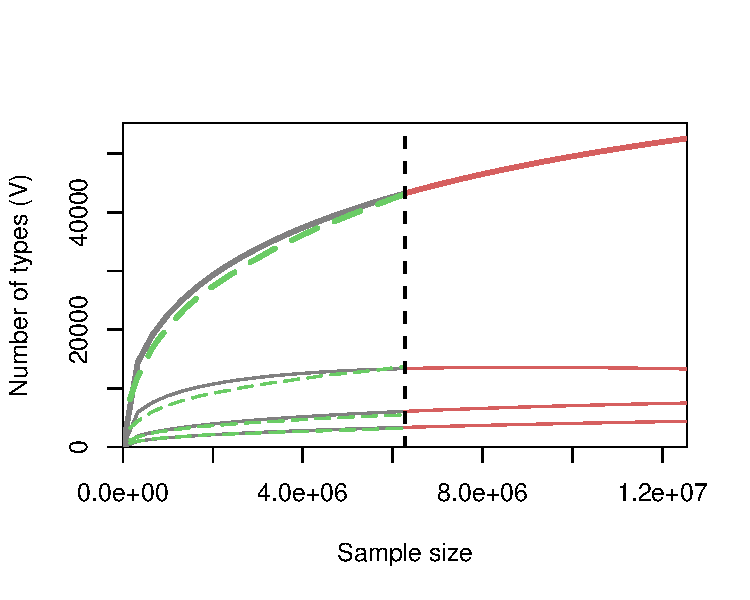
\includegraphics[scale=1]{figures/df.growth.intrextr-3.5.pdf}
    \caption{The type-token growth curves based on the LLM corpora show the increase in lexical richness as the sample size gets larger. The four curves show four different lexical richness measures (y-axis) on interpolated (solid grey), extrapolated (solid red), and observed (dashed green) sample size (x-axis), as based on a finite Zipf-Mandelbrot Large Numbers of Rare Events Model \citep[LNRE model, see][]{evert_simple_2004}. The four lexical richness measures are from top to bottom: total numbers of types, numbers of types that occur at most 3, 2, and 1 times (i.e., tris legomena $V_3$, dis legomena $V_2$, and hapax legomena $V_1$).}
    \label{fig:df.growth.intrextr}
  %\end{minipage}
  \hfill
\end{figure}


More generally, we can also investigate this pattern by inspecting the balance of high and low-frequency words as indicated by Zipf's law (i.e., word frequency is proportional to rank). This proportion in natural language corpora is never completely constant, so comparing the pattern across corpora can be interesting \citep[see, e.g., ][]{baayen_analyzing_2008, piantadosi_zipfs_2014, baayen_word_2001}. Figure \ref{fig:rankplot-normal} shows that Zipf's law in the LLM corpus is generally steeper compared to childLex. Previously, similar comparisons of adult corpora showed the same pattern \citep[i.e., SubtLEX and Google Book corpus, ][]{brysbaert_impact_2016}. For the LLM corpus, the slope is steeper compared to childLex, indicating that the LLM corpus includes more high-frequency words and fewer low-frequency words. Again, this finding also indicates that the LLM-generated text is less rich.  

\begin{figure}[!htbp]
  \centering
%  \begin{minipage}[t]{0.9\textwidth}
    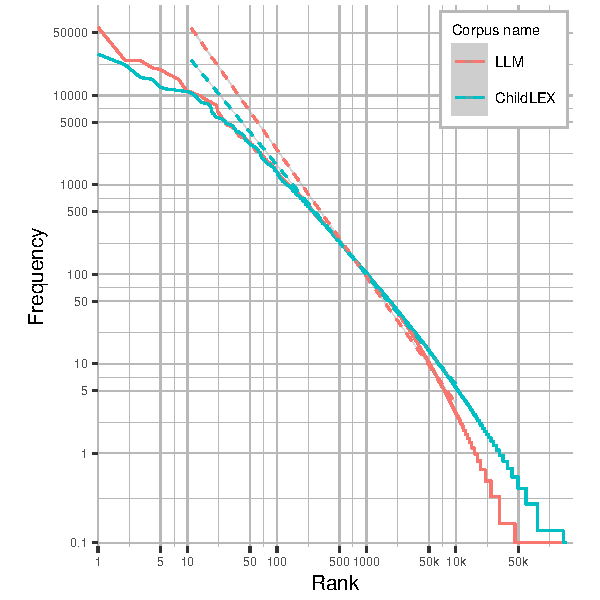
\includegraphics[scale=1.5]{figures/rankplot-normal-3.5-2.pdf}
    \caption{Zipf's law plot shows frequency count on the y-axis and frequency rank on the x-axis with linear regression lines (dashed lines) for both the LLM and ChildLex corpus. The slopes are fitted to words with a frequency between 10 and 10,000. The LLM slope is more negative, indicating a higher occurrence of highly frequent words and a lower occurrence of low frequent words.}
    \label{fig:rankplot-normal}
  %\end{minipage}
\end{figure}


Despite apparent differences, such as in lexical richness, we find a correlation between word frequency measures from childLex and the LLM corpus (r = .88 for frequency per million and r = .69 for log frequency per million, see Figure \ref{fig:cor1}). For computing log frequency, we used a kind of Laplace transformation (i.e., $\log\left(\frac{(1 + \text{frequency}) \times 10^6}{\text{corpus\_size}}\right)$; see Supplement for a comparison of different transformations and see \cite{heister_dlexdb_2011, van_heuven_subtlex-uk_2014} for similar procedures and discussion). The cone shape of the scatter plot (see Figure \ref{fig:cor1}) indicates that lower frequency measures are noisier (more variable) than higher word frequency measures, which makes sense, given the lower numbers of observations for low-frequency words. The relatively symmetric shape indicates that this noise is similarly distributed between both corpora. The correlation remains .88 when we include all words that do not occur in the other corpus (i.e. frequency of 0). The correlation based on log frequency also stays the same. The high correlation and the scatter plot illustrate the high similarity of the two measures. Comparing word frequency in this way also allows us to look at the words that differ in frequency the most in both directions. In the LLM corpus, words that are more frequent sometimes result from spillover effects from the most likely predominant English training data. For example, the German word "namens" is used more often in the LLM corpus than in childLex (i.e., 1414 vs. 31 per million). This could directly have "spilled over" from the typical phrase to start a story in English: "There was an X called Y" even though "namens" is not typically used in this context in German. This result is similar to the observed losses in lexical and morphological richness in automatic machine translation \citep{vanmassenhove_machine_2021}. The word frequencies that stand out in childLex are typically associated with narrative storytelling. This finding is unsurprising, as the LLM corpus comprises only summary-like texts. childLex contains some very common words that we would have expected in the LLM corpus. There is no clear explanation for these patterns, but some seem to indicate that childLex contains more colloquial style words (e.g., “offenbar”). Table \ref{notin} shows the most common words from both corpora that do not appear at all in the other corpus. In this table, the LLM column contains only names, which is a result of the way some common first names were removed from childLex but were kept in the LLM corpus. Unfortunately, we were not able to reconstruct the procedure for removing given names that were used for childLex. The supplemental information contains a more extensive analysis of such differences. 


\begin{figure}[!htbp]
  %\centering
  \centerline{
  %\begin{minipage}[t]{0.9\textwidth}
    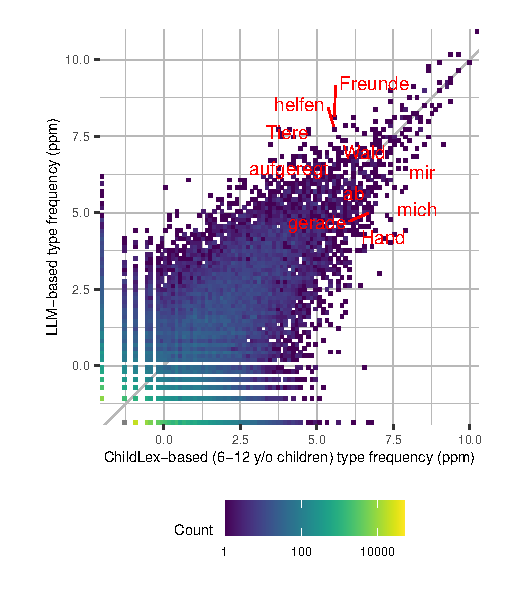
\includegraphics[width=1\textwidth]{figures/scatterplotexp1.pdf}}
    \caption{Correlation between LLM type frequency (y-axis) and childLex type frequency (x-axis; dark gray line). The labels show the top five differences on both sides (x-y and y-x). The color gradient of the dots represents the number of data points each dot represents.}
    \label{fig:cor1}
  %\end{minipage}
\end{figure}

% latex table generated in R 4.3.0 by xtable 1.8-4 package
% Thu Oct  5 12:26:55 2023
\begin{table*}[!htbp]
\caption{The top frequent words that occur in only one of both corpora, for all word lengths, and words with more than 10 characters. Some very common childLex words like "\textit{offenbar}" (\textit{evidently}), "\textit{rasch}" (\textit{quickly}), "\textit{Hoffentlich}" (\textit{Hopefully}), and "\textit{guckte}" (\textit{looked}) do not occur in the LLM corpus at all. Instead of "guckte" or "gucken", words like "angeguckt" and "abgucken" do appear in the LLM corpus. Also, common first names have been removed from childLex, but not from the LLM corpus.}
\centering
\begin{tabular}{rllll}
  \hline
 & childLex & childLex $>$10 & LLM & LLM $>$10 \\ 
  \hline
1 & daß & Hoffentlich & Max & nahegelegenen \\ 
  2 & 1 & Brombeerkralle & Mia & Schulvampire \\ 
  3 & offenbar & Hosentasche & Tim & Tantenschreck \\ 
  4 & rasch & Augenbrauen & Lisa & SkaterBande \\ 
  5 & Eigentlich & Zeigefinger & Lena & ParkSheriffs \\ 
  6 & ehe & SternenClan & Anna & Lesefähigkeiten \\ 
  7 & Gleich & Olchi-Kinder & Emma & Schafgäääng \\ 
  8 & Hoffentlich & eingefallen & Tom & SchmuddelHund \\ 
  9 & glaub & kopfschüttelnd & Müller & Inselschüler \\ 
  10 & guckte & unwillkürlich & Lina & verwirklicht \\ 
   \hline
\end{tabular}
\label{notin}
\end{table*}


\subsubsection*{Evaluating an LLM- based measure of word frequency using reading performance}

For the reading performance-based evaluation of the LLM word frequency measure, we used an existing dataset with reaction time data from a lexical decision task \citep{schroter_developmental_2017}. The dataset contained 1152 words. The words were selected in such a way that almost every word occurred in childLex and that the low-frequency words (e.g., < 10 per million) accounted for only 25\% of the words (in childLex, low-frequency words account for 95\% of the words). The correlation between LLM word frequency and reaction time ranged between .33 (grade 1), to .51 (grade 6), while childLex word frequency correlated between .36 (grade 1) to .58 (grade 6), see Figure \ref{fig:cormat_devel} for a correlation matrix. Both childLex and LLM word frequency correlated lower with adult reaction time (e.g., .47 and .39, respectively, for older adults). The LLM-childLex correlation was .76 for this subset of words, which is considerably larger than the correlation for the complete corpora (which was .63; see section above). 

We compared a linear regression model that included LLM word frequency measures based on the complete corpus to models that included multiple alternative word frequency measures. These other measures included childLex and two adult-directed corpora, a book-based corpus \citep[DWDS][]{heister_dlexdb_2011}, and a subtitle-based corpus \citep[SUBTLEX][]{brysbaert_word_2011}. These models also controlled for a number of other factors that potentially affect reading performance, but this is of no interest to the current study: OLD20 \citep[e.g., ][]{yarkoni_moving_2008,hawelka_beyond_2013}, age of acquisition \citep[e.g., ][]{weekes_effects_2006}, letter length \citep[e.g., ][]{gagl_sources_2015, huestegge_oculomotor_2009, marinus_variability_2010, zoccolotti_word_2005}, as well as phoneme count, uni-, bi- and trigram frequency. Note for the final analysis, we removed the phoneme count, uni-, bi-, and trigram frequency parameters due to high Variance Inflation Factors \cite{fox_generalized_1992}. When removed, all Variance Inflation Factors of the remaining predictors have been below 5, indicating low co-linearity \citep[i.e., see][for a similar procedure]{gregorova_access_2023}. After calculating the effect sizes from the linear model, we estimated the model fit based on the Akaike Information Criterion \citep[AIC, ][]{akaike_new_1974}. To estimate the AIC, we compared the model to a baseline model without a word frequency measure. Higher AIC differences indicate increased model fit when we added word frequency to the baseline model (see supplement Figure A4 for an analysis based on incrementally increasing text sizes for the estimation of the LLM word frequency). 

We found that the AIC difference is largest for the LLM word frequency for young readers (Grade 1-4; see Figure \ref{fig:modelcomprt}), indicating that the LLM word frequency measure describes the word frequency effect in young readers best. For Grade 6, we found that the SUBTLEX word frequency measure, which relied on subtitles from films and TV shows, had the highest model fit increase. Finally, the book and newspaper-based word frequency measures from the DWDS corpus showed the highest model fit in young and old adults (see Figure \ref{fig:modelcomprt}A; see Supplemental Table \ref{effsize} for a detailed description of model estimates, effect sizes, and the R squared metric). When the word frequency increases from 1 to 1000, the predicted response time decreases by about 250 ms.

\begin{figure}[!htbp]
    \centering
    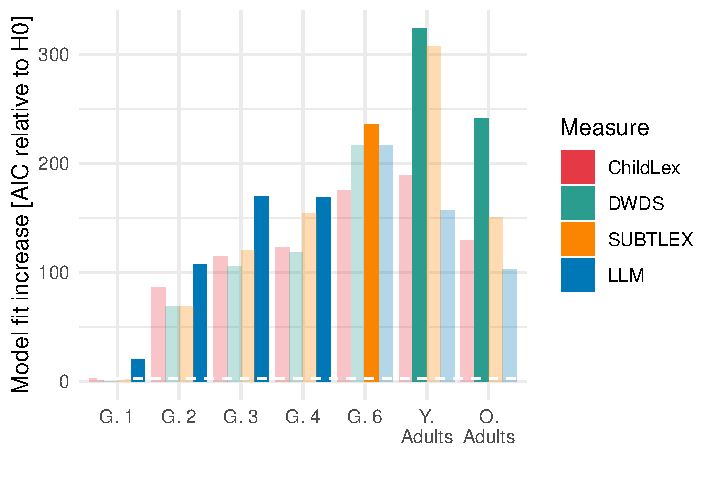
\includegraphics[scale=1]{figures/exp1_modelcomp.pdf}
    \caption{Evaluation of the word frequency effect on reading performance (lexical decision times) of beginning readers (Grades 1, 2, 3, 4, and 6), young and old adults. AIC difference is based on an analysis comparing the word frequency effect across LLM, childLex, DWDS, and SUBTLEX word frequency measures for all age groups. The models with the highest fit for each group are highlighted (i.e., the largest AIC difference). Note that G. abbreviates Grade; Y., Young; O., Old. The white dashed line indicates the threshold for a significant model fit increase.}
\label{fig:modelcomprt}
\end{figure}

The finding that LLM word frequency describes the word frequency effect in children best is accompanied by a reduction in effect size. When comparing the effect sizes of the word frequency effects between LLM and childLex word frequency, we found that for LLM word frequency, effect size tended to be smaller in grades 2-4 (see Figure \ref{fig:ef_size}A). Inspecting the scatter plots (as shown exemplarily in Figure \ref{fig:ef_size}B and C) shows that the reduction in effect size is the result of the low frequency measures and the words that have not been included in the LLM corpus but do exist in childLex. Indicating that these words have a crucial role here.

\begin{figure}[!htbp]
    \centering
    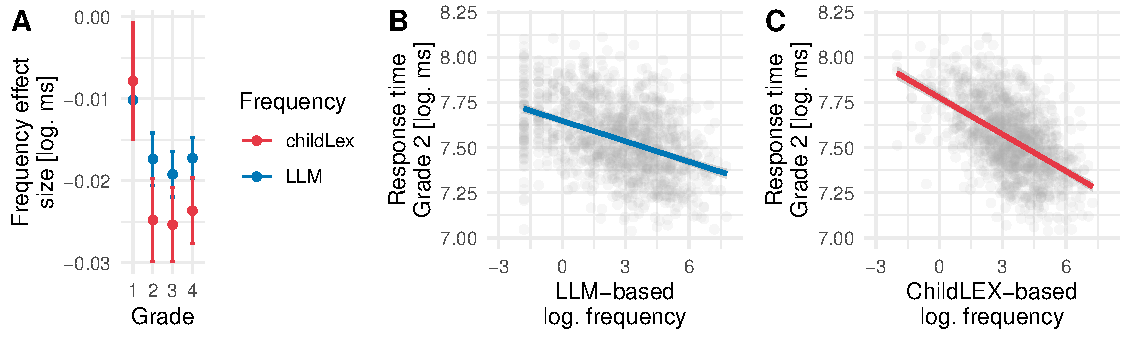
\includegraphics[scale=.8]{figures/exp1_ef_size.pdf}
    \caption{Evaluation of the word frequency effect size on reading performance (lexical decision times) of beginning readers (Grades 1, 2, 3, and 4). (A) Effect sizes with 95\% confidence intervals for log-transformed lexical decision response times of the young readers of grades 1-4 comparing the word frequency effect measured based on the LLM and childLex corpora. (B) Exemplary scatter plot including linear regression line showing the word frequency effect on lexical decision times in grade 2 readers based on the LLM and (C) childLex corpora.}
\label{fig:ef_size}
\end{figure}


\subsection{Summary: Experiment 1}

Word frequency measures based on LLM corpora explain more variance in lexical decision reaction times compared to traditional word frequency measures based on books. We generated a corpus based on multiple LLM prompts. In each prompt, we asked the model to compose a text for children in age-specific language. Critical for the evaluation was that we used the book titles from an established German corpus based on children's books \citep[childLex; ][]{schroeder_childlex_2015}. This enabled a more direct comparison between the word frequency measures from the original childLex corpus and the LLM corpus. There were three main findings: (i) The LLM corpus had a lower lexical richness (i.e., a lower number of distinct words), and relatively frequent words comprised a more significant part of the LLM corpus. (ii) LLM word frequency correlated strongly with childLex word frequency, showing a substantial similarity of the measures, although both corpora had a substantial number of words specific for one corpus. (iii) In reading-performance-based evaluations, we found that the LLM word frequency describes the performance of younger readers better than word frequency measures based on published children's books. Together, the present study indicates that LLM-based corpora do represent word frequency, despite the substantial differences compared to traditional corpora. Furthermore, this initial exploration indicates that the corpus resulting from the LLM text that is asked to generate text for children can especially well describe the word frequency effect in young readers.  


\section{Experiment 2}

We conducted a second experiment to investigate two of the most critical findings from Experiment 1. First, we found that the lexical richness of the LLM corpora was much lower than in childLex. Thus, we investigated how increasing the temperature parameter of the LLM influences the lexical richness of the corpus. Second, we investigated how the prompt design, implemented to generate text specifically for children, influenced the model fit to reading performance data from children grades 1-4. To investigate the combination of these two factors as well, we generated four additional corpora for experiment 2: two corpora generated with child-directed and two generated with adult-directed prompts, of which each had the same and one an increased temperature value (i.e., 0.5 and 0.9). Together, these four corpora included: (i) \textit{Child-Directed \& Low Temperature (ChLT)}. This corpus was based on the same prompts and the same temperature setting, a reproduction of the corpus from Experiment 1. (ii) \textit{Child-Directed \& High Temperature (ChHT)}. (iii) \textit{Adult-directed \& Low Temperature (AdLT}, as well as (iv) \textit{Adult-directed \& High Temperature (AdHT)}.

We expected lower model fits on children's reading performance for the word frequency effect based on the adult-directed LLM corpora, which would show that the LLM is indeed capable of producing text directed to children. We expected higher model fits for the reading performance data with child-directed LLM corpora and the other way around with adult-directed corpora. For temperature, we expected that a higher temperature increases lexical richness and potentially the model fit in reading performance. However, in Experiment 1, the lexically richer corpus (childLex) resulted in lower model fits in reading performance.  

Compared to Experiment 1, we increased the size of both child-directed LLM corpora to $\sim$ 23 million words (going from $\sim$ 6 million in Experiment 1) in order to approximate the size of childLex. We expect this to increase the number of overlapping words with childLex and to increase the reliability of the low frequency measures \citep{gernsbacher_resolving_1984}. This should also lead to more precise measures of lexical richness, which may be more important for a high temperature setting. 


\subsection{Methods}

We prompted the model to generate twenty texts with a low temperature setting of 0.5 and a high temperature setting of 0.9 for five age groups, resulting in the generation of 200 texts for each book. Using this method, we collected 5,500 child-directed texts for the low and the high temperature setting. 

We used the same prompt as in Experiment 1 except for the temperature (max. value for GPT-3.5-turbo: 2.0). Please note that the higher the temperature setting, the greater the chance of hallucinations. In initial explorations, a temperature above 1.0 resulted in frequent hallucinations, such as changing the names of the main characters in the story (e.g., Ferdinand instead of Fred). The higher temperature could also lead to incorrect changes to the plot of a book. This is why we decided to set the temperature to 0.9 in the high temperature condition and leave the same value as in Experiment 1: 0.5 in the low temperature condition. 

Although the parameter “max\_tokens” was set to 4000, again, the generated texts were much shorter, averaging about 278 words per text for the high temperature conditions and about 270 words per text for the low temperature conditions. 

Like Experiment 1, we compared the new LLM corpora with childLex \cite{schroeder_childlex_2015}, allowing us to inspect the lexical richness compared to a book-based corpus. Furthermore, we compared the DWDS word frequency measure and the LLM word frequency measure to determine which measure fits best. 

We used the log-transformed lexical decision response times of the DeveL dataset to inspect if the child-directed prompts resulted in a better description of word frequency in child- and adult-directed prompts to better descriptions of word frequency effects in adults. Note that to simplify this analysis, we grouped the child reading performance data for grades 1-4 together, as well as the data for the young and old adults. We omitted the adolescent group from Grade 6, since, as evident from Figure \ref{fig:modelcomprt}, the pattern was not fitting with the adults yet and already different from the younger readers. This is because the adolescents were the only group to show a preference for subtitle-based word frequency. 


\subsection{Results}

\subsubsection*{Word frequency distributions and lexical richness}

Table \ref{freqComp2} shows that all four crossed temperature and target audience conditions generally result in more unique types and lemmas compared to the LLM corpus from Experiment 1 (see Table \ref{freqComp}). Still, childLex is much richer than all LLM corpora. For the adult-directed LLM corpora, the higher number of unique types, compared to the LLM corpus from Experiment 1, is plausibly due to the adult-directed audience prompt change creating a richer vocabulary (i.e., see \textasciitilde 46,000 in Experiment 1 vs. \textasciitilde 71,000 and \textasciitilde 84,000 in the adult-directed LLM corpora). For the child-directed corpora, it is likely that the increase in unique types is due to a larger corpus size (i.e., see \textasciitilde 46k in Experiment 1 vs. \textasciitilde 85k and \textasciitilde 111k in the child-directed corpora from Experiment 2). For the child-directed corpora, the \% of hapax tokens (i.e., \% hapax legomena across all tokens, meaning the percentage of tokens in the corpus that occur only once) was lower compared to Experiment 1 (.12\% and .18\% vs. .25\%). This is also plausibly due to a larger corpus size, as the number of hapax legomena does not increase substantially for larger sample sizes (see the differences in slopes of Figures \ref{fig:df.growth.intrextr} and \ref{fig:df.growth.intrextr2}. The \% of hapax legomena across all types or all unique lemmas remained relatively constant with a larger corpus size (Types: Exp. 2: 33.56\% vs. Exp. 1: 33.03\%; Lemmas: Exp. 2: 33.00\% vs. Exp. 1: 33.09\%). Furthermore, the high temperature setting has a stronger influence on the \% of hapax types than having an adult target audience. In other words, the temperature setting more strongly influenced the percentage of words used only once, compared to the target audience. This can be illustrated by comparing percentages: 38.21\% for the child-directed LLM corpus with high temperature vs. 33.56\% for the corpus with low temperature is a larger difference than 34.69\% for the AdLT vs. 33.56\% for the ChLT corpus. Taken together, generating texts with a high temperature setting increased the lexical richness. However, the richness was still substantially lower than the lexical richness of the book-based childLex corpus (48.74\% Hapax types vs. $<$ 38.21\% in the LLM corpora). 

% latex table generated in R 4.2.2 by xtable 1.8-4 package
% Fri Jun 14 15:42:25 2024
\begin{table}[!htbp]
\caption{Size and descriptive statistics for the 4 LLM corpora from Experiment 2 compared to childLex. Ad \& Ch: adult- and child-directed, LT \& HT: low and high temperature.}
\centering
\begin{tabular}{lrrrrr}
  \hline
    Measure & childLex & AdLT & AdHT & ChLT & ChHT \\ 
  \hline
n Books & 500 & 500 & 500 & 500 & 500 \\ 
  Tokens & 9,850,786 & 7,191,531 & 7,368,921 & 23,320,466 & 23,887,118 \\ 
  Types & 182,454 & 71,423 & 83,921 & 84,978 & 110,603 \\ 
  Lemmas & 117,952 & 52,528 & 61,318 & 63,552 & 82,126 \\ 
  \% Hapax tokens & 0.90 & 0.34 & 0.44 & 0.12 & 0.18 \\ 
  \% Hapax types & 48.74 & 34.69 & 38.21 & 33.56 & 38.21 \\ 
  \% Hapax lemmas & 48.30 & 34.82 & 38.13 & 33.00 & 37.05 \\ 
  \% Tokens $>$ 4 & 97.89 & 99.41 & 99.29 & 99.79 & 99.71 \\ 
  \% Types $>$ 4 & 26.53 & 40.51 & 37.26 & 42.48 & 37.38 \\ 
  \% Lemmas $>$ 4 & 27.91 & 40.26 & 37.13 & 42.82 & 38.10 \\ 
   \hline
\end{tabular}
\label{freqComp2}
\end{table}

Using the growth curves from extrapolated sample sizes, we also see that the lexical richness in both adult-directed corpora was higher than in the child-directed corpora (see Figure \ref{fig:df.growth.intrextr2}). The number of types at around 20 million tokens ($2 \times 10^7$) is around 90,000 types for the AdLT corpus and 75,000 types for the ChLT corpus. Likewise, it is about 105,000 types for the AdHT corpus and only 95,000 types for the ChHT corpus (i.e., roughly an increase of 10-15,000 types for the adult-directed corpora). These differences are lower compared to the temperature manipulation (90,000 vs. 105,000 types in adult-directed corpora and 75,000 vs. 95,000 types in child-directed corpora). At 10 million tokens, childLex already has more than double the number of types (about 80,000 types for AdLT, 90,000 types for AdHT, 60,000 types for ChLT, and 70,000 types for ChHT). 

This pattern is also confirmed by comparing the relation between word frequency and rank for the three new conditions, like in Figure \ref{fig:rankplot-normal} from Experiment 1 (see Supplemental Figure \ref{fig:rankplot-normal2}). The three new conditions all fall between the curves from Experiment 1 and the curve based on childLex. The AdHT curve matches childLex most closely. 

\begin{figure}[!htbp]
  %\centering
  \centerline{
  %\begin{minipage}[t]{0.9\textwidth}
    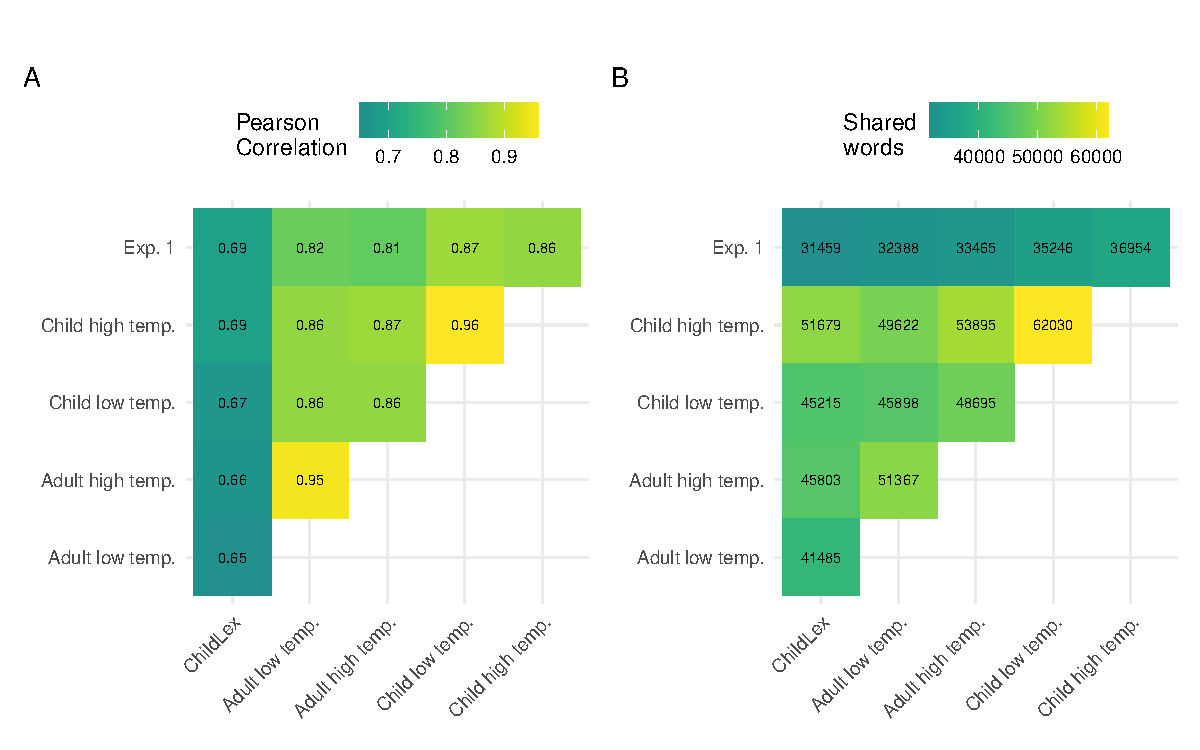
\includegraphics[width=1.1\textwidth]{figures/combined_plotc.pdf}}
    \caption{(A) Pairwise correlations between word frequency measures derived from the LLM corpora and childLex. (B) Numbers of shared words between corpora.}
    \label{fig:combined_plotc}
  %\end{minipage}
\end{figure}

The correlation between LLM and childLex word frequency was slightly smaller than the correlation we found in Experiment 1 ($r = .69$ vs. $.67$, see \ref{fig:combined_plotc}A). Word frequency from Experiment 1 correlated most strongly with those from the reproduction condition ($r = .87$). Figure \ref{fig:combined_plotc}B shows the varying numbers of shared words on which the pairwise computed correlations are based. We find higher correlations for the corpora with the same vs. different target audience, irrespective of temperature (see Figure \ref{fig:combined_plotc}A). In contrast, as we showed above, the \% hapax words across types or lemmas are more similar within vs. between temperature settings, illustrating the higher lexical richness due to increased temperature. Correlations involve a comparison of word frequency, while comparing lexical richness measures does not. Thus, with respect to correlations, the audience for which the LLM was generated matters more. 

The percentages of shared words show the same pattern observed for the correlations (see Supplemental Figure \ref{fig:heatmap}): The same target audience leads to more overlapping words compared to using the same temperature setting. Also, the ChHT corpus contained the highest percentage of words from childLex (33\%, see the first column for the child high temp. row in Figure \ref{fig:heatmap}). This suggests that prompting for a child target audience results in a better overlap with childLex compared to prompting for an adult audience and also that the higher temperature results in more recovered words. Also, compared to the 20\% shared words of Experiment 1, this marks a notable increase. Vice versa, childLex contained the most words from the AdLT corpus (58\%, see second column for the childLex row), probably because this corpus was the smallest with the least types. The overlap between the LLM corpora ranged between 33\% and 73\%. This indicates that corpus size, temperature, and target audience do result in relatively different types.  

The words in the LLM corpus that do not occur in childLex are very similar to those from Experiment 1 for both the low and high temperature conditions. ChildLex words that do not occur in the LLM corpus are now different, which is plausible, given the larger corpus from Experiment 2. The words that the LLM corpus misses seem varied, and include capitalized words for starting sentences such as Immerhin (anyway), see Supplemental Tables \ref{words-chlt} and \ref{words-chlt-low}, or Mich (mine), see Supplemental Tables \ref{words-chht} and \ref{words-chht-low}. It is plausible that such words will occur in even larger LLM corpora. Generally, the differences again illustrate that the LLM text is less narrative and uses a less varied sentence structure. 


\begin{figure}[!htbp]
  %\centering
  \centerline{
  %\begin{minipage}[t]{0.9\textwidth}
    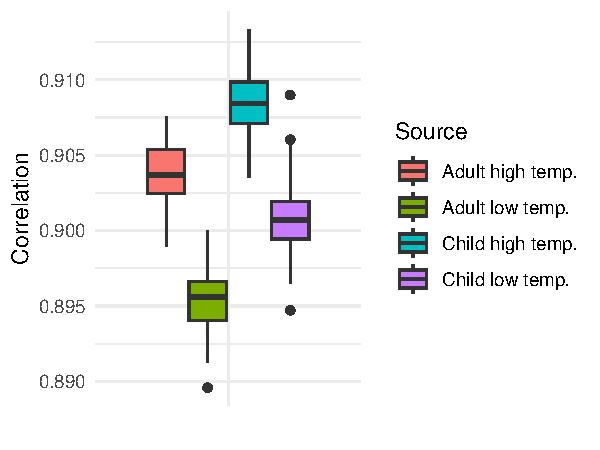
\includegraphics[width=.5\textwidth]{figures/boxplot-split-pearson.pdf}}
    \caption{Split half reliability estimates showing Pearson correlations.}
    \label{fig:reliablity}
  %\end{minipage}
\end{figure}

We also estimated the split-half reliability of the LLM corpora (see Fig. \ref{fig:reliablity}). We correlated LLM word frequency from a random selection of texts based on half of the book titles with the texts based on the other half of the book titles, and repeated this 100 times. The correlations are thus based on correlating corpora that are based on completely different book titles with each other. Correlations range from an average of .895 for adults low temperature to .908 for the ChHT corpus (averaging across 100 random splits of 2x250 books). These correlations are higher compared to the LLM-childLex correlation, which was .62. The result, therefore, shows that the word frequency tables remain very similar across different book titles relative to childLex. Furthermore, correlations were higher in the high compared to the low temperature conditions, and they were higher in the child-directed compared to the adult-directed corpora. 


\subsubsection*{Evaluating LLM-based word frequency measures based on reading performance}

We computed the correlations between LLM word frequency and the lexical decision reaction times for the subset of words from the Devel dataset \citep{schroter_developmental_2017}. These correlations were almost identical (maximally .02 difference) for both the ChLT (the reproduced corpus) and the ChHT corpus. Both adult-directed corpora had lower correlations across all grades (.04 - .07 lower; see Figure \ref{fig:cormat_devel} for a correlation matrix). Correlations with adult reaction times were similar across the new conditions (maximally .01 difference for older adult reaction times). The correlations for the child-directed corpora also did not increase compared to Experiment 1 and were also comparable across conditions (maximally .02 difference), which we also found for the correlations between complete corpora (see section above). 

Next, we determined if age-specific corpus generation allows a better estimation of the word frequency effect on the reading performance of the specific age group. Similar to Experiment 1, we estimated model fit increase (i.e.,  AIC) in relation to a baseline model (i.e., without a word frequency parameter included) with adult-directed LLM word frequency for adult and child reading performance data and vice versa (see Fig. \ref{fig:modelcomprt2}A). We found that age-specific corpora had a higher model fit specifically for the reading performance of the group they were directed to. Effect sizes were numerically larger with overlapping confidence intervals when a child-directed LLM word frequency measure was used for the child reading performance data compared to an adult-directed LLM word frequency measure and vice versa (see Fig. \ref{fig:modelcomprt2}B).

Furthermore, when inspecting the temperature manipulation, it is clear that an increase in temperature increases both model fit (see Fig. \ref{fig:modelcomprt2}A) and effect size (see Fig. \ref{fig:modelcomprt2}B). This effect size increase, in contrast to the pattern found in Experiment 1, is expected to result from increasing the lexical richness of the underlying corpus. Compared to the finding of Experiment 1, where the word frequency measure derived from the lexically richer childLex corpus had a lower model fit but higher effect size, we find that an increase in temperature increases both effect size and model fit. 

\begin{figure}[!htbp]
  %\centering
  \centerline{
  %\begin{minipage}[t]{0.9\textwidth}
    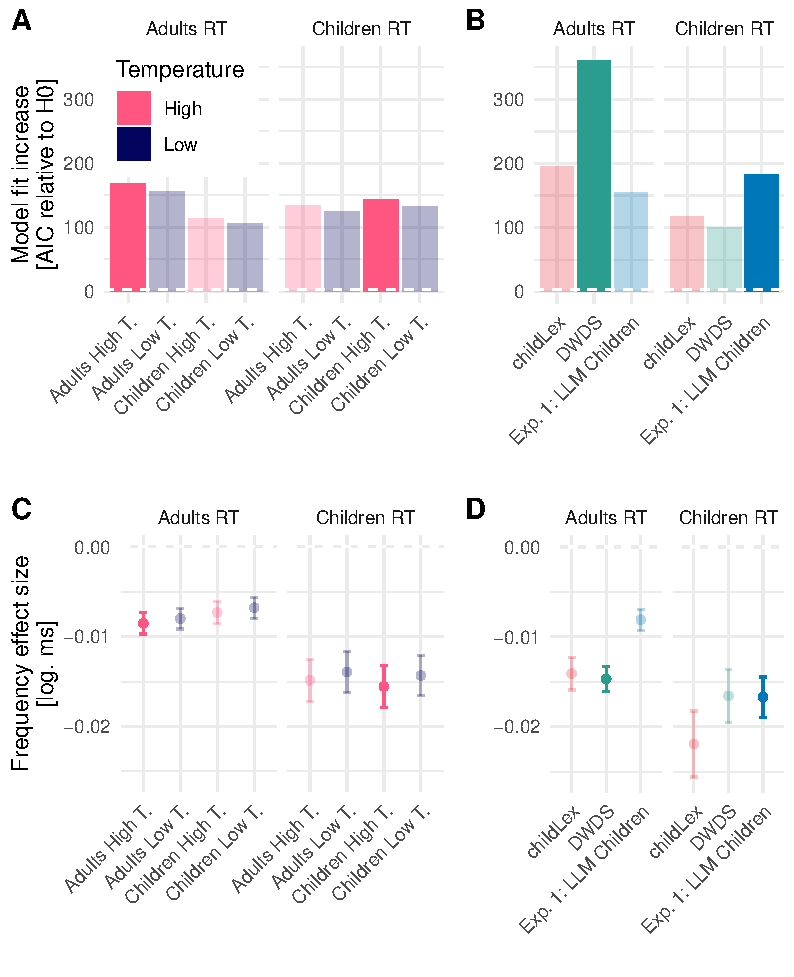
\includegraphics[width=.8\textwidth]{figures/exp12-new-col.pdf}}
    \caption{Model comparison and effect size results for adult and child reading performance data using (A) AIC for statistical model comparison based on the Experiment 2 corpora and (B) the Experiment 1 corpora as well as childLex and DWDS. Corresponding effect size estimates on log-transformed lexical decision response times from linear mixed effect regression models, including the 95\% intervals, are presented for word frequency measures of experiment 2 in (C) and Experiment 1 in (D). Note that high or low temperature is color-coded in red and blue in (A) and (C). The white dashed line in (A) and (B) indicates the threshold for a significant model fit increase. Model comparison results, measured in AIC points relative to a baseline model without a word frequency measure.}
    \label{fig:modelcomprt2}
  %\end{minipage}
\end{figure}


In addition, we compared the model fit results from the high temperature corpora (i.e., the best-fitting models from experiment 2) to alternative word frequency measures (see Fig. \ref{fig:modelcomprt2}). Again, we show the model fit increase based on the word frequency measures from the LLM corpus from Experiment 1, childLex, and DWDS, shown to have high model fit in adult reading performance. In comparison, we find that the child-directed LLM corpora have a higher model fit than the various book-based corpora. The inverse is the case for the adult-directed corpora. The most notable outcome here is that the LLM corpus from Experiment 1, even when generated with a low temperature setting, had the highest model fit. Also interesting for adults was that childLex had a higher model fit than the adult-directed LLM corpus. 


\subsection*{Summary: Experiment 2}

To summarize, in the second experiment, we replicated the main finding of Experiment 1: We showed that a word frequency measure derived from LLM corpora can be used to model the word frequency effect in reading effectively. Experiment 2 manipulated two more variables: 1) the LLM temperature parameter (high vs. low) to try to increase the lexical richness of the corpus, and 2) the target audience (adults vs. children) to investigate if this results in different word frequency measures. 

We found that a higher temperature increased the lexical richness of the corpora. Also, we found that higher temperatures resulted in higher model fits. In line with Experiment 1, we found evidence that LLM corpora can be tailored to a specific target audience. This finding is reflected in increased model fit.

We also observed several unexpected findings. First, lexical richness was still unlike the book-based childLex corpus. Also, book-based corpora (childLex and DWDS) showed higher model fits for adults compared to the adult-directed LLM corpora. Finally, we found that the child-directed corpus from Experiment 1 had a higher model fit than the larger and more lexically rich corpora from the second experiment. Here, we expect that this is due to changes in the underlying LLM that are outside our control (see detailed discussion below).


\section*{General Discussion}

In two experiments, we showed that word frequency measures based on LLM corpora can be used to model the word frequency effect effectively. For young readers, we find that child-directed prompts can be used to generate corpora and derive a measure of word frequency that explains more variance in children's lexical decision reaction times compared to a book-based word frequency measure \citep[childLex; ][]{schroeder_childlex_2015}. 

A comparison of effect sizes shows that LLM word frequency measures not only have a higher model fit but also indicate that the word frequency effect for children is potentially overestimated by book-based corpora. In contrast, adult-directed LLM corpora are better at explaining the word frequency effect than child-directed LLM corpora. However, book-based corpora resulted in higher levels of explained variance. We find that the LLM corpora, irrespective of size and temperature, generally have a lower lexical richness (i.e., a lower number of distinct words). Increasing the temperature parameter of the LLM does only slightly increase the lexical richness. Thus, the results indicate that LLM-based corpora can be used to derive an effective measure of word frequency. However, this comes with substantial differences and caveats, discussed below, compared to book- and subtitle-based corpora.  


\subsection*{Low richness of LLM corpora}

The central difference between our LLM corpora and childLex is that it includes fewer types, and frequent types occur more often. To a smaller extent, we increased lexical richness by promoting the LLM for adult-directed text and by increasing the temperature parameter of the LLM. Note that by increasing the temperature of the LLM, the "creativity" of the model output increases, resulting in meaningless text when increased to extreme values. Text generated with the temperature value of .9 (which we used in Experiment 2) was not easily distinguishable from text generated with the temperature value of .5 (used in Experiment 1).  

Explanations for the low richness of LLM corpora may be found in our prompt design (discussed below) but also in the nature of LLMs more generally. Typically, LLM performance suffers in, e.g., reasoning tasks \citep{razeghi_impact_2022} and when answering fact-based questions \citep{kandpal_large_2023} that involve low-frequency words \citep{oh_frequency_2024}. A high-frequency bias is plausible for multiple reasons, such as text comprehension being easier with high-frequency words. 

Another explanation may result from our prompt design. Word count limits prevent the generation of book-length text. We prompted the LLM multiple times to compose a summary for each book. This procedure allowed us to generate a substantial number of words related to the topic from each childLex book. The resulting text is very different from the original books in terms of style. LLMs may more often generate words central to a book (e.g., \textit{wand} in Harry Potter) and use fewer function words and word types that indicate direct speech, such as "sagt" (\textit{says}). Future efforts could include creating completely novel books (i.e., as shown \href{https://medium.com/@baen2810/ai-assisted-writing-of-a-book-cataclysm-67788412fb31}{here}) directed to a specific group to increase lexical richness and generate improved corpora. 

The results of Experiment 2 rule out that low lexical richness is the result of our child-directed prompt design (i.e., we added "for children" or "for adults" to the prompts). If the LLM corpora had the same size as childLex (10 million tokens), they would have had roughly less than half of the types (200,000 vs. 100,000 types). The lexical richness of childLex is roughly comparable to other existing adult-directed corpora. For example, \citet{baayen_word_2001}) reports also reports about 200,000 types for an adult-directed corpus containing 8 million tokens (a corpus of news articles from "The Independent" English newspaper). The low richness of LLM text is troubling when thinking about the use of LLM text in education \citep[see also ][]{kasneci_chatgpt_2023} and other contexts where lexical variety is important.

We did not attempt to optimize our prompt design to generate a narrative style with plausible narrative elements and structures. Our main objective was to evaluate the use of LLM text as a psycholinguistic resource for word frequency measurement. We were able to demonstrate a specific use case (i.e., model comparison between different measures of reading performance) without optimizing text quality characteristics. Summary-like text already achieves a selection of words and word frequencies that work. This is evidenced by the fact that we observed a moderately strong correlation between word frequency measures from childLex and the LLM corpus (.69 for log-frequency per million across \textasciitilde 50,000 words), which seems normal compared to previously reported correlations. For example, SUBTLEX-UK (an English subtitle-based corpus) correlated with .66 to the Children Printed Word Database (\textasciitilde 9000-word frequencies across 11000 English children books, \citep{van_heuven_subtlex-uk_2014}, albeit using a different but similar transformation of the word frequency counts. Together, LLM text does seem to be able to approach certain qualities of psycholinguistic resources. 

Beyond lexical richness, it is clear that the LLM text remains qualitatively different from human-written text because it is more stereotypical and does not utilize many narrative and rhetorical elements. Child-directed LLM text is less engaging and uses fewer narrative elements, including figurative language and rhetorical devices, when compared to child-directed books. Further, other LLMs do not appear to improve on this problem. \citet{kumarage_neural_2023} applied stylometric analyses to LLM texts and found that GPT 3.5 and 4 styles do not differ much from each other, relative to open-source LLMs. Although we used lexical richness as a measure to characterize these differences in comparison with a book-based corpus (childLex), it is necessary to perform more detailed comparisons with other corpora, not necessarily child-directed corpora, as well as study other lexical, grammatical, and semantic statistics, including entropy, complexity, word frequency profiles, embeddingss etc. \citep{hu_language_2024, dentella_systematic_2023, munoz-ortiz_contrasting_2024, wu_survey_2024}. More research is necessary to determine the literary capabilities of modern LLMs compared to humans. 

Finally, our findings show that larger corpora have a higher coverage, but the similarity increase to a classical book-based corpus is only incremental. Larger LLM corpora still contain fewer different words than childLex. This was the case when using higher temperatures, when generating larger corpora, or when targeting the text to adults. In addition, the overlap in terms of the percentage of shared words between different LLM corpora was not much higher compared to overlap with childLex. This seems to imply that LLMs are capable of producing numerous words, but that the proportion, with which they do so, compared to common words, is much lower than in human text corpora. Therefore, the vocabulary of LLMs does not seem to be the reason that is withholding LLMs from producing a level of lexical richness as childLex. 




\subsection*{Reading performance-based evaluation of LLM- and book-based word frequency}

We used the word frequency based on the five LLM corpora to estimate the word frequency effect on reading performance. We compared the model fit and effect sizes for different age groups, as young as in Grade 1 up to old adults, separately. In addition, we compared the LLM corpora with a set of established word frequency measures like childLex, but also to two word frequency measures based on adult-directed corpora: DWDS \citep{heister_dlexdb_2011} and SUBTLEX \citep{brysbaert_word_2011}. We found that for Children, the LLM word frequency had the highest fit. For adolescents, the SUBTLEX word frequency, based on film subtitles, had the highest fit. For adults, the book-based DWDS corpus had the highest fit. 

In an experiment designed to generate child- and adult-directed corpora, we found that for child reading performance, child LLM word frequency had the better fit, and for adults, adult word frequency had the better fit. This finding indicates that when we specify the target audience in the prompt of the LLM, the output of the model indeed adapts. Thus, the child-directed word frequency measure includes words that are well recognized by kids more often. In addition, several words that are included in the book-based corpus are not included in the LLM corpus. This results in the prediction of high response times. 

Overall, we find that the child-directed word frequency measure not only describes the word frequency effect in young readers better, but also indicates that the size of the effect could be lower than expected. Book-based word frequency measures showed higher effect sizes, potentially overestimating the word frequency effect in young readers. In contrast, for the adult LLM word frequency measure, we found that the book-based corpora better fitted the word frequency effect but also showed higher word frequency effects. Noteworthy is that the word frequency effect size is comparable for young and adult readers when measured with the most appropriate age-specific word frequency measure. 

This pattern offers three critical insights: (i) for young readers, LLM word frequency best describes reading performance and variance over and above classical book-based frequency. This finding could indicate that the word frequency effect that describes the process of accessing the mental lexicon \citep{brysbaert_word_2018, brysbaert_word_2011, gregorova_access_2023} is better defined based on a corpus that has fewer types that are more frequent. (ii) The size of the frequency effect could be lower than expected from book-based word frequency measures and is constant over age groups when the appropriate word frequency measures are used for estimation. 
%The highly expected smaller lexicons in Grade 1 readers \citep[e.g.][]{segbers_how_2017} are reflected in the better fit of LLM word frequency measures when the corpus is small. This observation suggests that investigating the word frequency effect at the beginning of literacy acquisition demands an estimation of word frequency based on smaller corpora with child-specific content, in our case, generated by an LLM. 
(iii) For adolescents in Grade 6, the subtitles-based measure was best, while the adult book- and newspaper-based corpus was the best fit for the younger and older adults. This finding indicates that the child-specific prompts resulted in a corpus that best describes visual word recognition performance in young readers. In contrast, the book-based corpora better described the performance of adult readers.  

What could explain the surprisingly good fit of LLM word frequency to reading performance data? One possibility is that the complexity of the LLM is actually improving the word frequency measures. Normally, raw word frequency is considered an important factor in reading performance. However, word recognition and processing necessarily rely on the distances and similarities to other words based on how they are embedded in their semantic networks. These mental representations may be more closely mimicked by LLM word frequency compared to human corpus-based word frequency. LLMs use architectural principles such as transformers and attention heads, which ideally capture the most important similarities between words. Traditional corpus-based word frequency measures come directly from original documents with a document-specific semantic structure, resulting in word frequency estimations that depend much on the style and content that the writer used for that document's purpose. Although 500 books is a lot, this is, of course, only a fraction of the amount of training data that LLMs use. The intermediate processing by LLMs, i.e., training on extremely large amounts of text, adds a layer of "regularization" to word occurrence that seems to help capture the processing cost of words. 

Overall, the results suggest that LLM-based measures of word frequency better explain variability in lexical processing by young readers compared to the book-based word frequency. With this finding in mind, it seems possible to generate linguistic corpora for other less-well-represented groups and languages \citep[][]{gagl_eye_2022, blasi_over-reliance_2022}. Extensive experimentation is needed, as described above, to study such extrapolation and generation of new resources, currently unavailable but desperately needed. LLM corpora for underrepresented languages and groups could help in broadening psycholinguistic research, not only involving the most commonly studied populations and high-resource languages \citep{henrich_weirdest_2010, blasi_over-reliance_2022}. 

Importantly, by showing the potential of the approach, this study also highlights potential dangers. Extrapolating to groups underrepresented in the training data will likely be affected by the Western bias in currently used training data \citep{atari_which_2023}. Simply adding multilingual training data does not even necessarily improve multilingual LLM performance, possibly due to capacity limits \citep{chang_when_2023}. The specific LLM used here is not specifically developed to perform well in multilingual tasks and, indeed, reaches worse performance compared to specific models in multilingual tasks \citep{lai_chatgpt_2023}. At the same time, German is a high-resource language that performs better than, e.g., Chinese or Vietnamese across several multilingual tasks \citep{lai_chatgpt_2023}. Thus, practical uses may conflict with current model biases, particularly for low-resource and non-Western languages. Although little is known about LLM performance in low-resource languages, the approach described here could be a first step. 


\subsection*{Limitations and future research}

In our second experiment, we validated the assumption that generated child-directed text indeed differs from generated adult-directed text. We also ensured that the low richness was not due to a too low temperature setting. The next step is to select more transparent and less complex models, potentially in toy examples, with all parameters known. We used a non-transparent, very large, and continuously changing model. When a model is not transparent, it is not possible to know for sure what kind of training data the model has seen. \citet{liesenfeld_opening_2023} list a number of recent LLMs that do provide information on openness dimensions, including training data. Also, mechanistic explanations become impossible when complexity is so high that the model becomes a black box \cite{bender_dangers_2021}. For studying cognitively plausible ways in which word frequency approximates reading times, LLMs that are only as large as developmentally plausible are necessary (see \citep{feng_is_2024, tan_devbench_2024, hu_auxiliary_2024} for recent work in this direction). Furthermore, performance changes in unpredictable ways for non-transparent LLMs that are being trained continuously, using so-called fine-tuning. In the present study, LLM word frequency from Experiment 1 resulted in much better model fits (AIC > 100) compared to the reproduction condition from Experiment 2. One potential explanation is that certain model parameters changed in the elapsed time between these experiments. It is plausible that performance changed due to continuous and large-scale reinforcement learning with human feedback \citep[RLHF][]{bai_training_2022, chung_scaling_2024, perez_red_2022, ziegler_fine-tuning_2020}. In this process, LLMs are trained to better align with user requirements. This alternative optimization leads to a necessary trade-off between performance on next-word prediction and performance on alignment. Using a model that does not change over time would circumvent such issues. 

With respect to text comparison methods, the lexical richness measures and word reading times we used here are simplistic qualities of text compared to the cultural, social, and ethical themes and pedagogical considerations underlying the text of children's books. This study does not discuss the higher-level semantics or syntax of the books analyzed here. In addition, the study does not investigate whether LLM text can be used to assess these qualities. The text generated for this study is available, see \href{https://osf.io/wmuvj/?view_only=06ba6b0ec23248df8a1418add4da05a0}{osf.io} and can be used for such investigations. We showed that explained variation in word reading times depends on how lexical properties are quantified, including word frequency. We showed that LLM text contains atypical patterns, such as the spillover effects from English to German or numerous words found only in the LLM corpus but not in the book corpus. Such patterns indicate that generated text cannot substitute human text, particularly not in settings involving vulnerable participants (e.g., in the context of school or the wider public). 

LLM word frequency shows a smaller effect and explains more variance in reaction times compared to "valid" child book-based word frequency. These findings are difficult to explain within the current approach. How can cognitively implausible LLM word frequency be more informative about processing measures than "cognitively plausible” children’s book-based word frequency? This is an empirical question with many possible answers. Such an answer also involves studying how adults infer which words are known by children, how well they can infer children's vocabulary, and if authors, on purpose, add unknown words to their books with a pedagogical purpose (i.e., to increase the vocabulary of children). 


\section*{Conclusions}

Astonishingly, word frequency measures based on child-directed LLM text are similar to existing resources such as childLex and LLM-based word frequency measures can model the word frequency effect on reading performance of young readers better. The estimated effect size turns out to be smaller. This opens up new possibilities for investigating the word frequency effect, i.e., one of the strongest and most replicated effects in psycholinguistics research \citep{brysbaert_word_2018} and beyond \citep{gregorova_access_2023}. 

Still, caution is essential when trying to understand the possibilities of LLMs for language development research. LLMs deviate in crucial ways from natural language acquisition pathways. The different nature of LLMs results, on the one hand, in surprisingly different patterns of language use (c.f. \citep{vanmassenhove_machine_2021}, and on the other hand, in patterns of word processing cost that closely follow empirical data from children. The result is a first approach mapped out to quantify and compare how the elements of LLM text correlate with metrics from classic corpora and human behavior.


\section*{Declarations}

\textbf{Funding} This research was supported by the University of Cologne. 

\textbf{Conflicts of interest} We have no conflicts of interest to disclose. 

\textbf{Ethics approval} Not applicable. 

\textbf{Consent to participate} Not applicable. 

\textbf{Consent for publication} Not applicable. 

\textbf{Availability of data, materials, code, and supplementary materials} See our OSF repository: \href{https://osf.io/wmuvj/?view_only=06ba6b0ec23248df8a1418add4da05a0}{osf.io}. We will update this link when this paper is published. 



%\printbibliography
\newpage
\bibliographystyle{apacite} 
\bibliography{gpt.bib}
\newpage

\appendix
% TODO, merge other suppl stuff here in one file to allow crossrefs

\section{Additional Analyses}

\subsection{Experiment 1}

\subsubsection{Most different words}

Table \ref{words-least} shows the top words from the one corpus that appear the least often in the other corpus. 

% latex table generated in R 4.3.0 by xtable 1.8-4 package
% Thu Oct  5 12:26:56 2023
\begin{table*}[!htbp]
\caption{The top frequent words that occur the least often in the other corpus, for all word lengths, and for words with more than 10 characters.}
\centering
\begin{tabular}{rllll}
  \hline
 & ChildLex & ChildLex $>$10 & LLM & LLM $>$10 \\ 
  \hline
1 & Ganz & Wahrscheinlich & Jack & Sattelschlepper \\ 
  2 & Wieso & widersprach & Charaktere & Mäusepension \\ 
  3 & Wahrscheinlich & blitzschnell & Brownie & Schulgespenst \\ 
  4 & Bestimmt & Snorkfräulein & Brumm & aufgewecktes \\ 
  5 & Soll & verächtlich & Poppins & unvergessliches \\ 
  6 & verzog & irgendeinem & Zaubermaus & akzeptierten \\ 
  7 & kreischte & anschließend & Sattelschlepper & Korallenschatz \\ 
  8 & quer & irgendjemand & Fips & Abschlussfeier \\ 
  9 & presste & Zaubereiministerium & Hoppel & verantwortungsvoll \\ 
  10 & Meinst & Entschuldige & Mäusepension & unzertrennliche \\ 
   \hline
\end{tabular}
\label{words-least}
\end{table*}

\clearpage

\subsubsection{Litkey}

We redrew the scatter plot from the main text using a corpus containing texts written by children themselves \citep{laarmann-quante_litkey_2019} instead of text written for children \cite{schroeder_childlex_2015}. This corpus is much smaller, but the resulting figure, see Figure \ref{fig:corlitkey}, shows the same pattern and the most differing words can be explained similarly as well. 

\begin{figure}[!htbp]
  %\centering
  \centerline{
  %\begin{minipage}[t]{0.9\textwidth}
    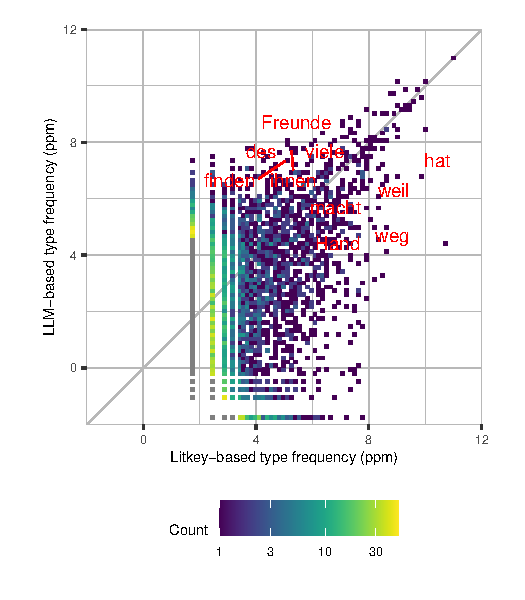
\includegraphics[scale=1.4]{figures/litkey.pdf}}
    \caption{The same as Figure 3 in the main text, but showing Litkey-based type frequency (x-axis). The pattern is similar, despite much less available data. }
    \label{fig:corlitkey}
  %\end{minipage}
\end{figure}

\clearpage


\subsubsection{Rank differences}

Figure \ref{fig:rankplot-difs} zooms in on the specific differences between childLex and LLM curves shown in Figure 2 from the main text, similar to \ref{fig:rankplot-normal}. Positive differences indicate a higher LLM word frequency, while negative differences indicate a lower LLM word frequency. Before rank 1,000, LLM words are roughly used more often, while after rank 1,000, LLM words are generally used less often. This finding again illustrates that the LLM uses high frequency words more often and low frequency words less often.  

\begin{figure*}[!htbp]
    \centering
    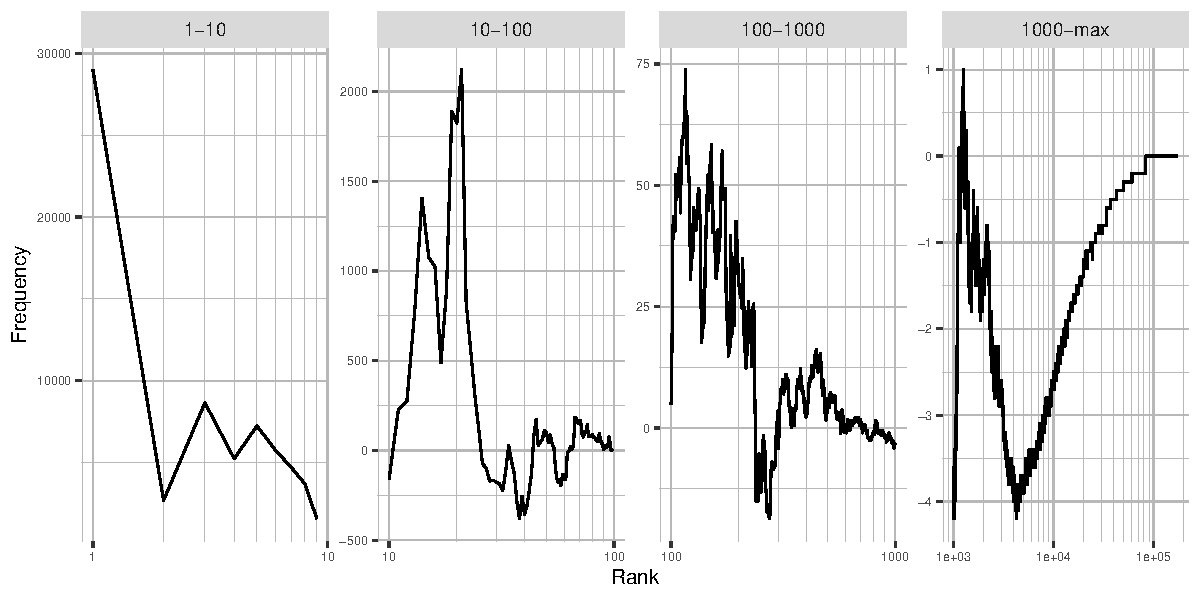
\includegraphics[width=\textwidth]{figures/rankplot-difs-3.5-2.pdf}
    \caption{Differences between word frequency calculated based on the LLM and ChildLex corpora (i.e., the difference between the curves from Figure \ref{fig:rankplot-normal}).}
    \label{fig:rankplot-difs}
\end{figure*}

\clearpage


\subsubsection{DeveL comparison}

\begin{figure}[!htbp]
    \centering
    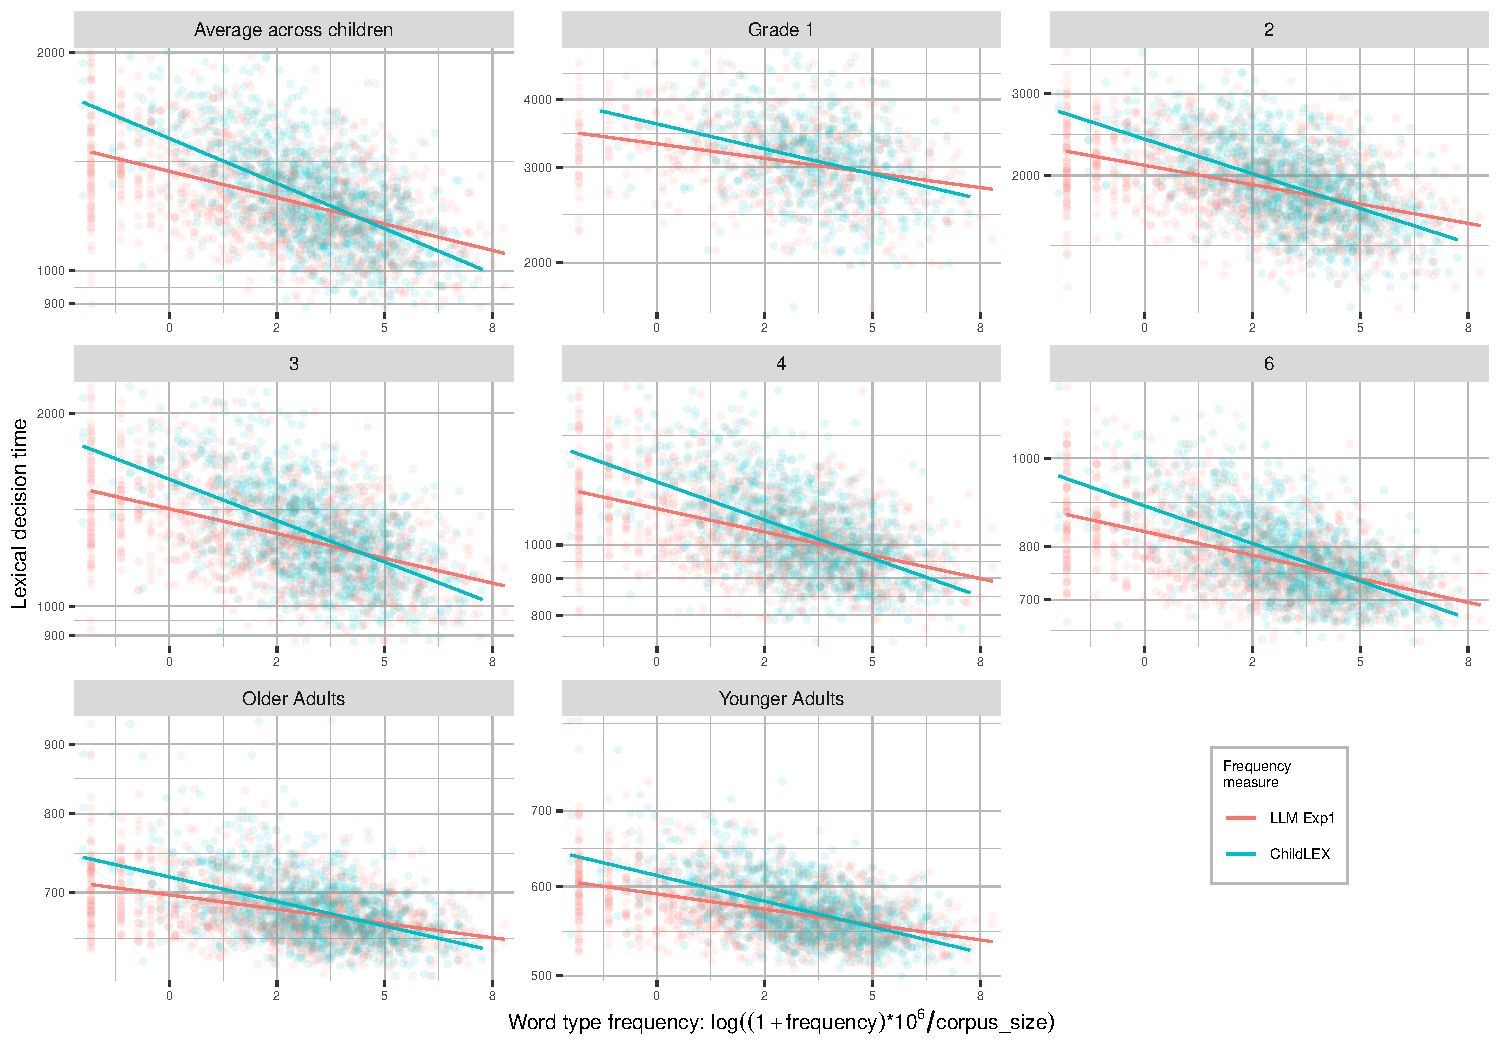
\includegraphics[width=\textwidth]{figures/exp18plus1-log.pdf}
    \caption{Relation between log reaction times (ms) with LLM and childLex log-frequency.}
\label{fig:rt-f-scatter}
\end{figure}

\clearpage


\subsubsection{Effect sizes}

% latex table generated in R 4.3.0 by xtable 1.8-4 package
% Mon Aug  5 11:24:23 2024
\begin{table}[!htbp]
\caption{Effect size estimates based on a subset of the DeveL data that excludes words with 0 occurrences in the LLM corpus. }
\centering
\begin{tabular}{lrrrrr}
  \hline
 & Estimate & SE & $t$ & $p$ & Adj. $R^2$   \\ 
  \hline
  Grade 1 \\ 
  LLM Freq. & -33.7 & 7.3 & 4.6 & \textbf{$<$ 0.001} & 0.6321 \\ 
  childLex & -22.1 & 12.0 & 1.8 & 0.066 & 0.6198\\ 
  Grade 2 \\ 
  LLM Freq. & -34.3 & 3.3 & 10.3 & \textbf{$<$ 0.001} & 0.6874 \\ 
  childLex & -48.1 & 5.3 & 9.1 & \textbf{$<$ 0.001} & 0.681 \\ 
    Grade 3 \\ 
  LLM Freq. & -25.6 & 2.0 & 12.7 & \textbf{$<$ 0.001} & 0.6562 \\ 
  childLex & -33.7 & 3.2 & 10.4 & \textbf{$<$ 0.001} & 0.6404 \\ 
      Grade 4 \\ 
  LLM Freq. & -19.6 & 1.5 & 13.3 & \textbf{$<$ 0.001} & 0.5699 \\ 
  childLex & -26.3 & 2.4 & 11.1 & \textbf{$<$ 0.001} & 0.55 \\ 
  \hline
\end{tabular}
\end{table}

\clearpage


\subsubsection{Robustness against sample size of the LLM-childLex word frequency correlation for the DeveL subset. }

To estimate the robustness of the correlation between LLM and childLex word frequency, we re-estimated the LLM word frequency based on subsets from the complete corpus, specifically for the words used in the DeveL dataset \citep{schroter_developmental_2017}. For this analysis, we started with the first LLM texts generated based on a prompt using the first book. After that, we successively added the texts from the next book and re-estimated the correlations for each subset (see Figure \ref{fig:partial_data}A). The curve shows a logarithmic increase in corpus similarity, indicating a substantial correlation increase of the two measures within the first 50 texts. After that, the increase in similarity is weaker, ending up at a correlation coefficient of just below .75. We tested whether the increase in similarity is indeed logarithmic. For this, we compared two correlations: The correlation between all correlation quotients (i.e., see y-axis in Figure \ref{fig:partial_data}A) and (i) the numbers of texts (i.e., see x-axis in Figure \ref{fig:partial_data}A) or (ii) the logarithm of the numbers of texts. The computed correlation for the linear number was lower (r = .71) than the correlation based on the logarithmic numbers (r = .94), indicating that the increase is indeed logarithmic  (Figure \ref{fig:partial_data}B also reports this correlation of .94 in the top left corner). The analysis shows that word frequency would not have been very different if we had used only half of the LLM corpus. It turns out that the correlation seems to keep increasing, but that it slows down with more text. 


\subsubsection{Model fit estimations based on partial corpus word frequency measures}

Here, we evaluated to what extent word frequency measures based on corpus subsets result in a lower model fit. Thus, we increased the corpus size (same as above), estimated the word frequency, and measured the model fit change when introducing the established word frequency measures compared to a model without the measure. We implemented this, starting with the texts from the first book. Ultimately, we can compare the absolute AIC difference values (i.e., AIC from the model with the new word frequency predictor minus the AIC based on the model without the predictor; the higher, the better the model fit) from all estimated word frequencies and all reading groups (1st-4th Grade, 6th Grade, young and old adults; N tests = 500; see Figure \ref{fig:partial_data}C). We rely on model comparison methods using linear regression models and the AIC, a measure optimal to investigate model fit change for newly introduced parameters. Note that a change in three AIC points is a significant model fit increase (i.e., the black horizontal line in Figure \ref{fig:partial_data}C and D; all AICs above show a significant increase in model fit).

The clear finding of this partial corpus analysis is that the reading performance can be explained better based on word frequency measures that we estimated from larger corpora (Figure \ref{fig:partial_data}C). We find an increase in the AIC difference in all age groups, although the trend is much smaller in the youngest readers from Grade 1 (compare correlations of the size of the corpus - N - and Grade 1 - G1 - in contrast to the more older readers in Figure \ref{fig:partial_data}B). Nonetheless, all analyses, except for the word frequency measures based on very small corpora (Number of books < 5) predicting the reaction times of Grade 1 readers, showed a significant increase in model fit. Correlations of AIC differences with increasing corpus size of all our groups of readers also showed that in Grade 1, the pattern differed from all other groups (Figure \ref{fig:partial_data}B). In addition, groups with similar age (e.g., Grade 2 vs. Grade 3) had higher correlations (r range from .96 to .99) compared to comparisons with substantial age differences (e.g., Grade 2 vs. old adults; r = .81). Finally, the partial analysis that estimated the AIC differences against a baseline model including childLex word frequency as a predictor, showed that only linear models that predicted the reaction times of young readers (Grade 1-6) had an additional model fit increase based on the inclusion of the LLM word frequency (see Figure \ref{fig:partial_data}D). Models describing adult data did not benefit from introducing the LLM word frequency measure. Also, we observed that for young readers, larger corpus sizes are needed for the word frequency measurement to produce a measure with higher descriptive power (Grade 1: 6 books; 2: 103; 3: 59; 4: 95; 6: 121; see Figure \ref{fig:partial_data}D).


\begin{figure}[!htbp]
    \centering
    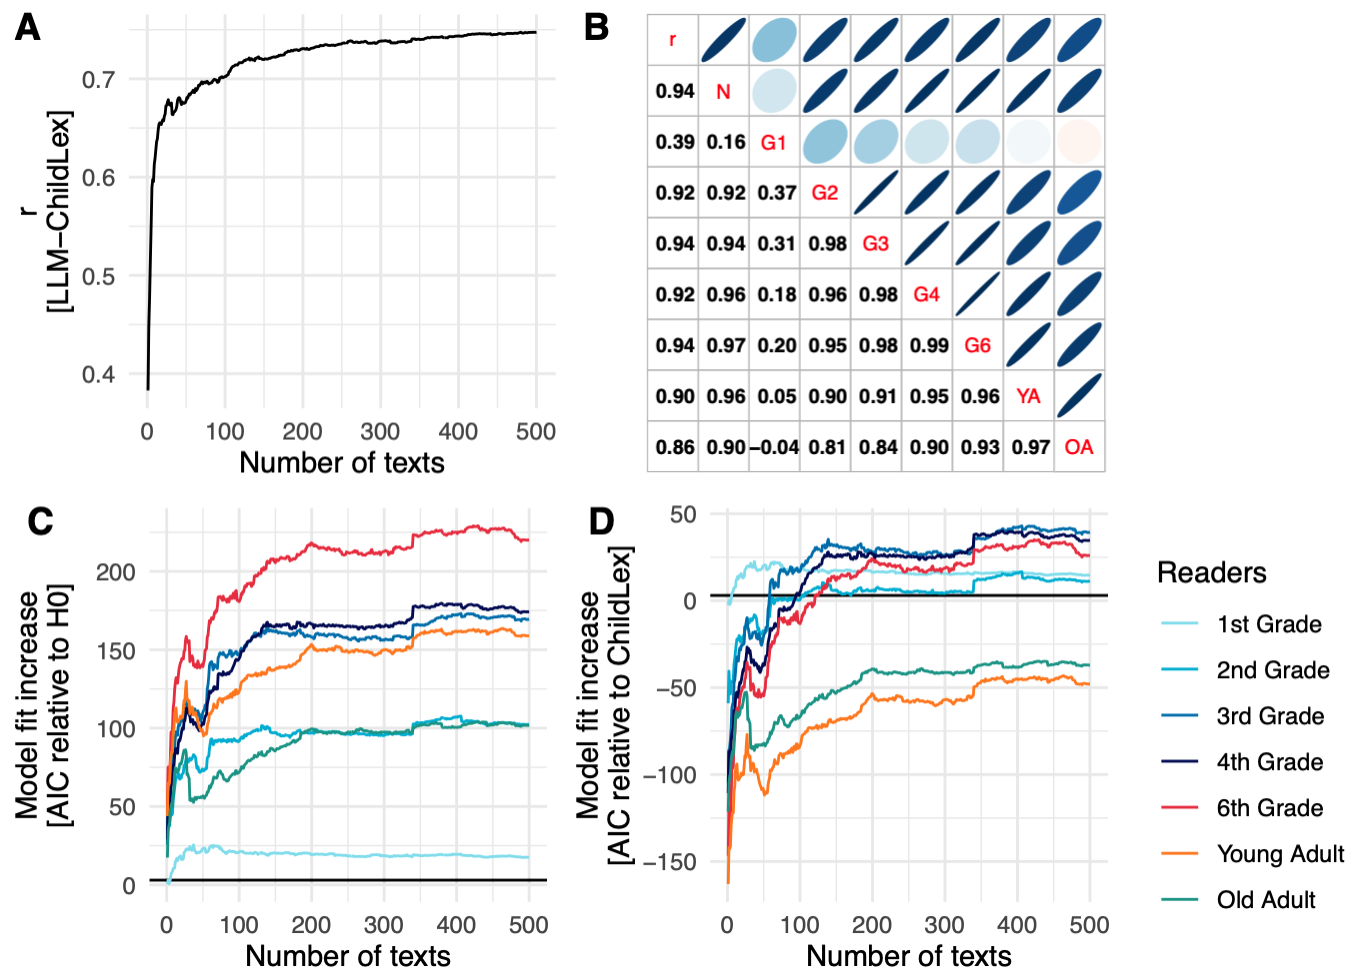
\includegraphics[scale=.30]{figures/partial_fig.png}
    \caption{Partial LLM corpus analysis. (A) Subset-based estimation of the correlation between LLM type frequency and childLex type frequency (y-axis). We estimated the correlation 500 times based on an LLM word frequency extracted from a corpus that included only the first book. After that, we included all generated text from one additional book until all books were included. Note that this analysis was implemented for the words used in the DeveL dataset. (B) Pearson correlation matrix investigating the partial data curves from A and C. \textit{r} represents the correlations from A; \textit{N} represents the log-transformed number of stories (i.e., x-axis from A, C, or D); \textit{G1-6}, represent the AIC differences from Grade 1 to 6 shown in C; \textit{YA} and \textit{OA} represent the young and old adults AIC differences shown in C. Lower matrix shows the correlation coefficient r and the upper matrix the color coded (blue: positive correlation; white: no correlation; red: negative correlation) correlation silhouettes (narrow silhouettes indicate high and wide silhouettes indicate low correlations). (C) AIC differences for linear mixed models of the DeveL reaction times. The models included word frequency measures estimated on a subset of the LLM corpus (i.e., same subsets as in A), which were compared to the model without a word frequency measure included, and (D) when the baseline model included childLex word frequency.}
    \label{fig:partial_data}
\end{figure}

For the evaluation based on reading performance, we used the lexical decision data of the DeveL dataset (i.e., response times of young readers from Grades 1-6, young and older adults). In the first analysis, we found that the model fit, in describing the response time data, increased when including a word frequency measure based on only a fraction of the full LLM corpus (N $<$ 10 texts) for all age groups. Nonetheless, increasing the corpus size also increased the model fit further. For all but Grade 1 readers, the increase in model fit with a larger corpus was highly similar to the increase in the correlation between LLM- and book-based corpora described above (r range: .86 - .94). The difference for Grade 1 was that model fit analysis peaked after about 10\% of the corpus, with an incremental decrease of model fit for word frequencies based on larger corpora (i.e., when N $>$ 100). 

Similarly, we compared the model fit increase for LLM word frequency based on partial corpora to a model that already included childLex word frequency. Here, we investigated whether the new LLM word frequency explains variance over and above traditional word frequency measures. Most notably, this was the case for the Grade 1 readers after only a fraction of the texts included (N $<$ 10). For Grades 2-6 readers, an increased model fit was found when the LLM corpus size was much larger (Grade 2: N $>$ 100; Grade 3: N $>$ 50; Grade 4: N $>$ 100; Grade 6: N $>$ 120). No additional variance was explained when the childLex word frequency was already included for the two adult groups. 
\clearpage


\subsubsection{Effect sizes}

% latex table generated in R 4.3.0 by xtable 1.8-4 package
% Mon Aug  5 11:24:23 2024
\begin{table}[!htbp]
\caption{Effect size estimates per grade.}
\centering
\begin{tabular}{lrrrrr}
  \hline
 & Estimate & SE & $t$ & $p$ & Adj. $R^2$   \\ 
  \hline
  Grade 1 \\ 
  LLM Freq. & -27.1 & 6.1 & -4.4 & \textbf{$<$ 0.001} & 0.6363 \\ 
  childLex & -25.1 & 11.4 & -2.2 & \textbf{0.028} & 0.6269\\ 
  Grade 2 \\ 
  LLM Freq. & -30.9 & 3.0 & 10.4 & \textbf{$<$ 0.001} & 0.6916 \\ 
  childLex & -50.0 & 5.1 & 9.8 & \textbf{$<$ 0.001} & 0.6886 \\ 
    Grade 3 \\ 
  LLM Freq. & -24.4 & 1.8 & 13.6 & \textbf{$<$ 0.001} & 0.6613 \\ 
  childLex & -37.0 & 3.1 & 11.8 & \textbf{$<$ 0.001} & 0.6495 \\ 
      Grade 4 \\ 
  LLM Freq. & -17.9 & 1.3 & -13.8 & \textbf{$<$ 0.001} & 0.5861 \\ 
  childLex & -27.7 & 2.3 & -12.2 & \textbf{$<$ 0.001} & 0.5734 \\ 
  \hline
\end{tabular}
\label{effsize}
\end{table}

\clearpage


\subsection{Experiment 2}

\subsubsection{Rank comparison}

\begin{figure}[!htbp]
  \centering
%  \begin{minipage}[t]{0.9\textwidth}
    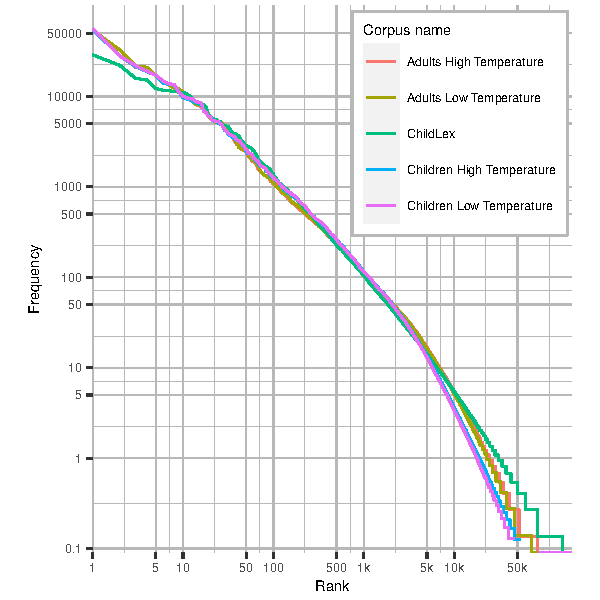
\includegraphics[scale=.7]{figures/rankf1-exp2.pdf}
    \caption{Overlap measured as percentage of retrieved words from one of both corpora. Overlap was defined as a word frequency > 0 for both corpora. The overlap percentages were computed by taking the number of words shared between the corresponding corpus listed on the left and bottom and dividing that number by the total corpus size of the corpus listed on the bottom row.}
    \label{fig:rankplot-normal2}
  %\end{minipage}
\end{figure}

\clearpage


\subsubsection{Corpus overlap}

\begin{figure}[!htbp]
  \centering
%  \begin{minipage}[t]{0.9\textwidth}
    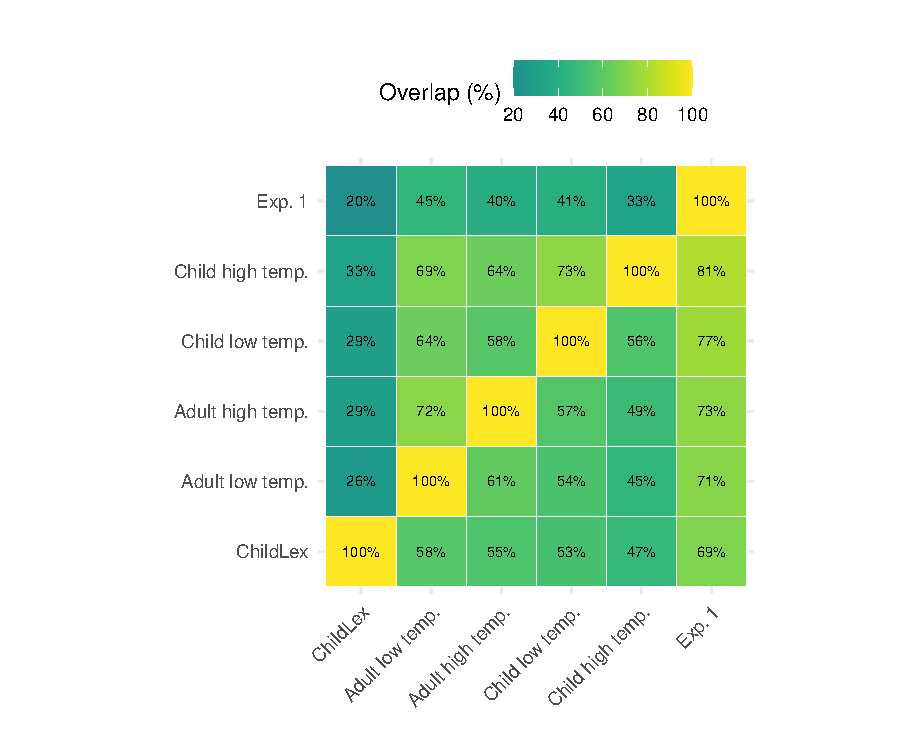
\includegraphics[width = \textwidth]{figures/heatmap.pdf}
    \caption{Zipf's law plot showing a stronger negative slope for the LLM corpus compared to ChildLex. The slopes are fitted to words with a word frequency between 10 and 10,000. }
    \label{fig:heatmap}
  %\end{minipage}
\end{figure}

\clearpage


\subsubsection{Type-token comparison}

\begin{figure}[!htbp]
  \centering
  %\begin{minipage}[t]{0.9\textwidth}
    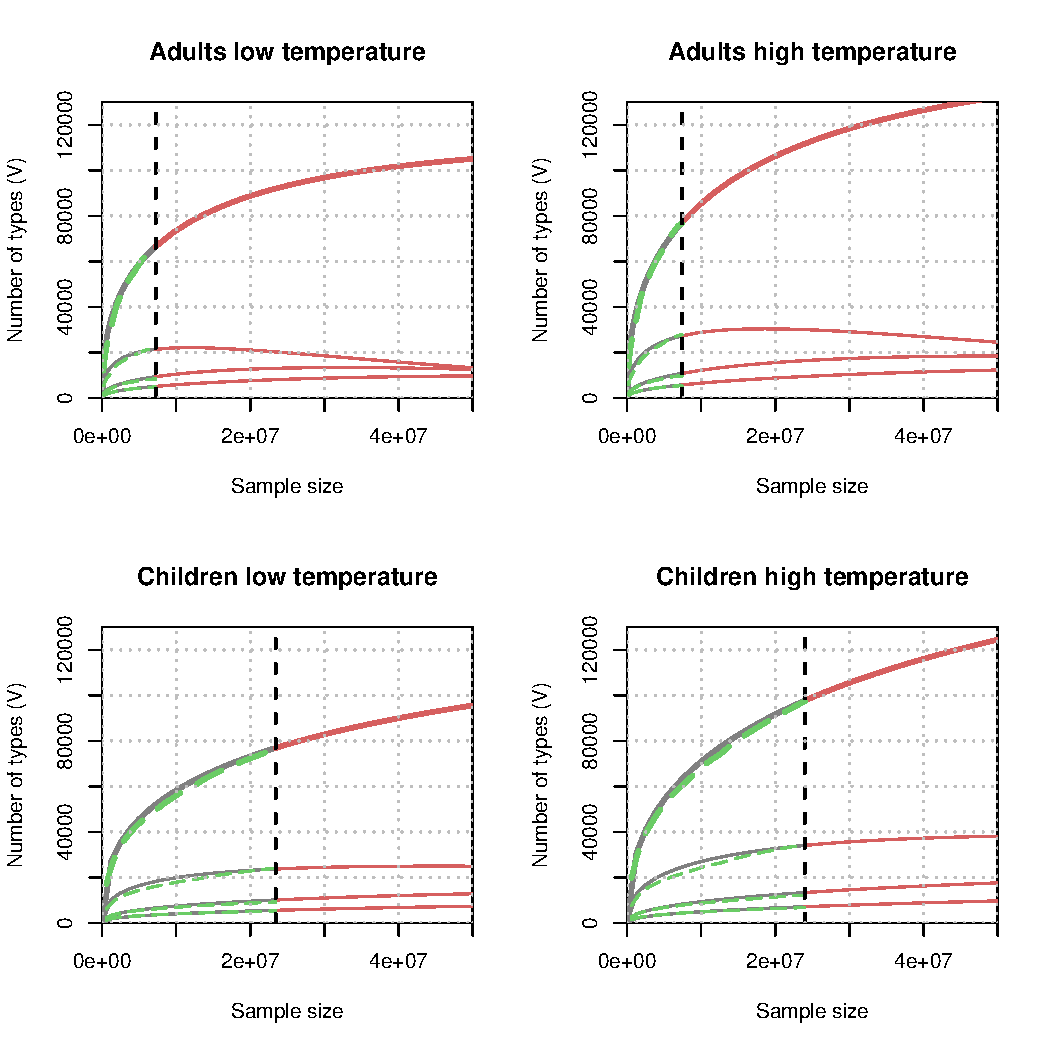
\includegraphics[scale=.8]{figures/vgc_plots_grid.pdf}
    \caption{Similar to Figure 1 (the type-token growth curve from the main text, these type-token growth curves show the dependency of the total number of unique types (y-axis) on inter- and extrapolated sample sizes (x-axis) for both adult-directed corpora (top), and for both child-directed corpora (bottom).}
    \label{fig:df.growth.intrextr2}
  %\end{minipage}
  \hfill
\end{figure}

\clearpage  


\subsubsection{Word frequency comparison across corpora}

\begin{figure}[!htbp]
  %\centering
  \centerline{
  %\begin{minipage}[t]{0.9\textwidth}
    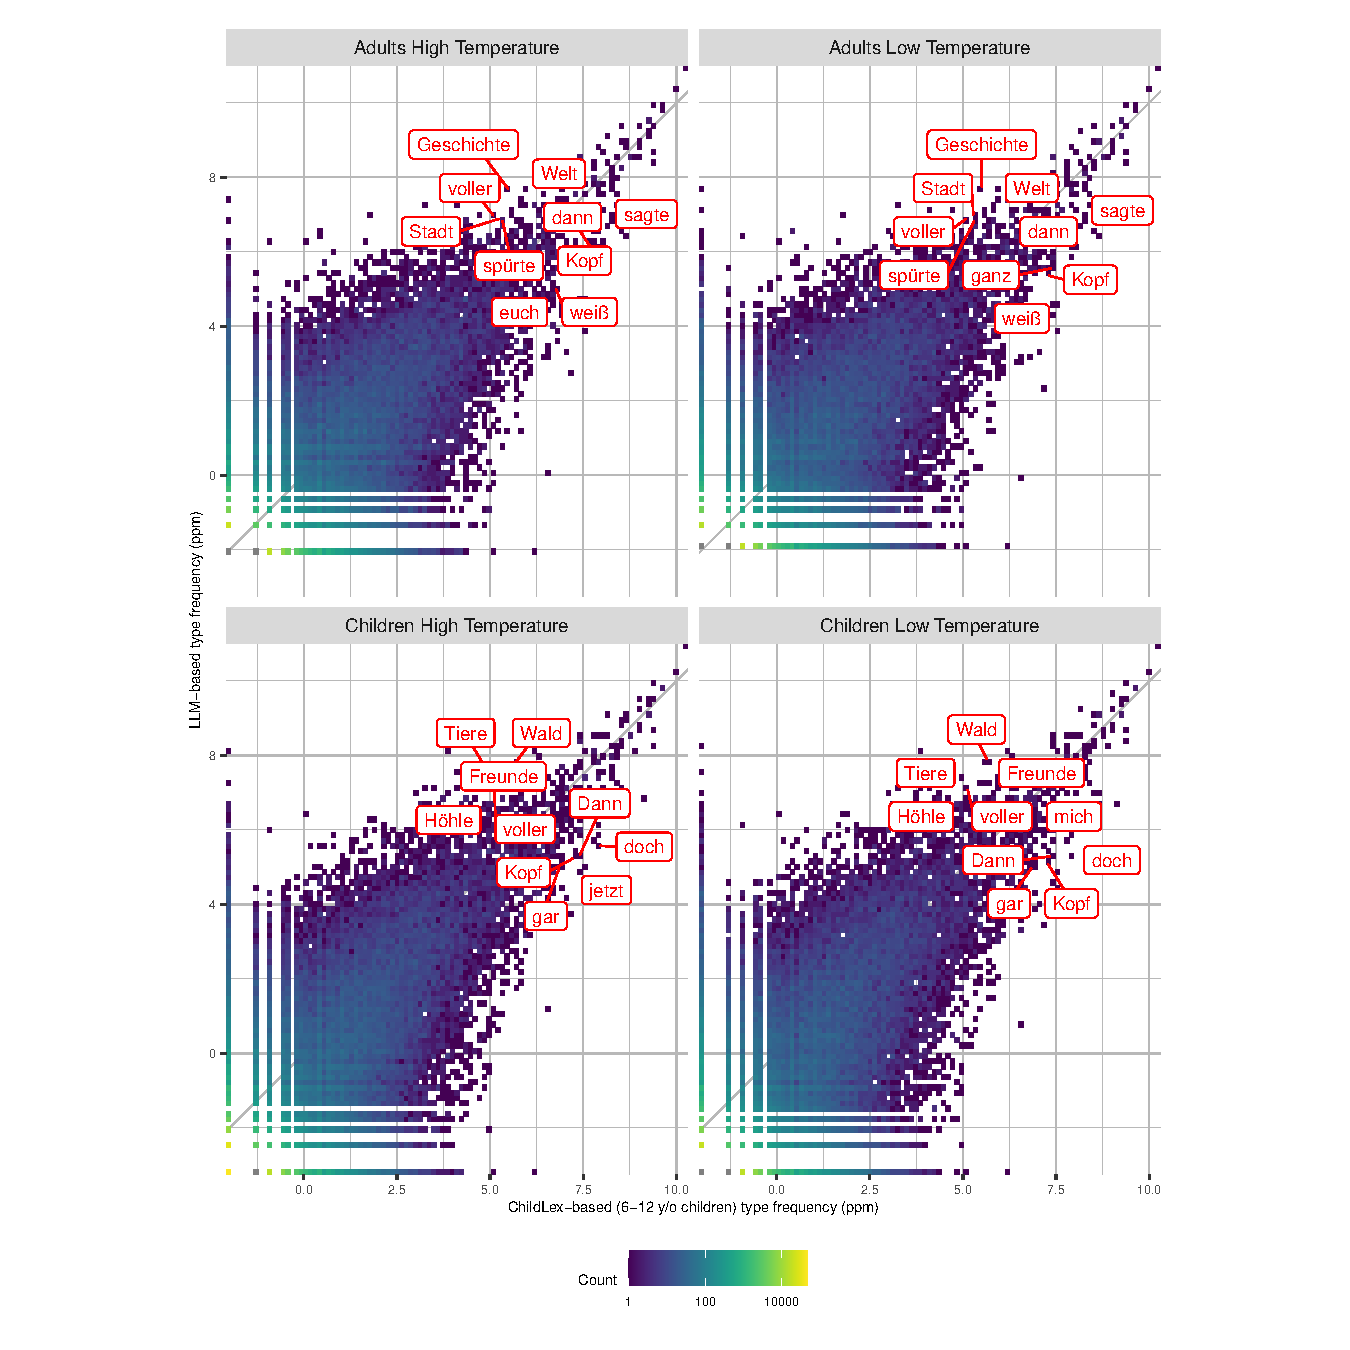
\includegraphics[scale=.7]{figures/scatterplotfacets.pdf}}
    \caption{Scatterplots between LLM type frequency (y-axis) and childLex type frequency (x-axis; dark gray line) for all four corpora from Experiment 2. The labels show the top five differences on both sides (x-y and y-x). The color gradient of the dots represents the number of data points each dot represents.}
    \label{fig:scatterplotfacets}
  %\end{minipage}
\end{figure}

\clearpage


\subsubsection{High frequency words comparison}

\begin{figure}[!htbp]
  %\centering
  \centerline{
  %\begin{minipage}[t]{0.9\textwidth}
    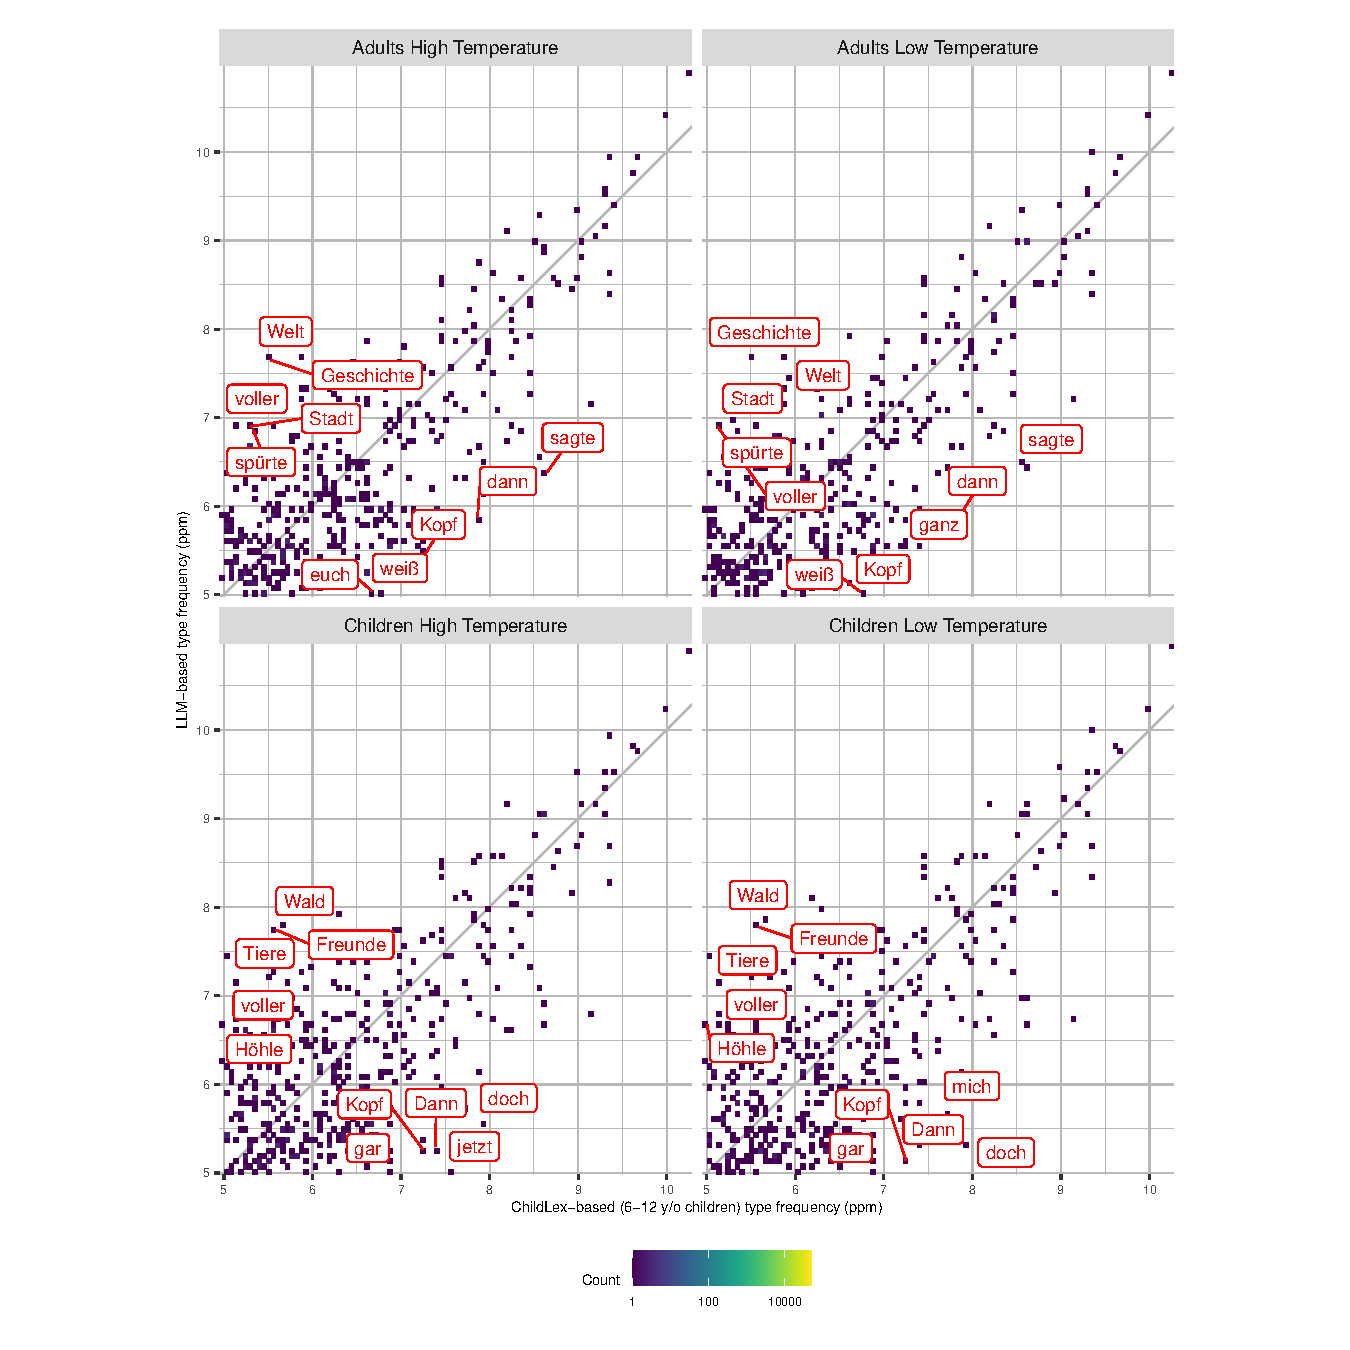
\includegraphics[scale=.8]{figures/scatterplotfacetszoom.pdf}}
    \caption{Zoomed in version of \ref{fig:scatterplotfacets}}
    \label{fig:scatterplotfacetszoom}
  %\end{minipage}
\end{figure}

\clearpage


\subsubsection{Word frequency transformation}

The histograms in Figure \ref{fig:histogram_plot_devel} show that 

\begin{equation}
\log\left(\frac{(1 + \text{frequency}) \times 10^6}{\text{corpus\_size}}\right),    
\label{eq:theone}
\end{equation}

is the most sensible transformation. Other options we considered included: 

\begin{equation}
\log \left( 1 + \frac{\text{frequency} \times 10^6}{\text{corpus\_size}} \right), 
- \log \left( \frac{1 + \text{frequency}}{\text{corpus\_size}} \right), 
\log \left( 1 + \text{frequency} \right) 
\label{eq:others}
\end{equation}

The first transformation of \ref{eq:others} (third row in Figure \ref{fig:histogram_plot_devel} results in a lower bound of 0 and an upper bound of 1 for normalized word frequency between 0 and 1. The resulting distribution collapses these values on this narrow interval, resulting in a skewed distribution. 

Furthermore, the transformations in Figure \ref{fig:scatter_plot2_devel} show the effect of corpus size on the transformed word frequency. For larger corpora, which include the child-directed LLM corpora and SUBTLEX, the non-normalized transformation ($\log \left( 1 + \text{frequency} \right)$) results in the strongest differences acrosss the corpora. 

Finally, the transformations in Figure \ref{fig:scatter_plot_devel} finally show the different handling of low frequency values. In particular, $\log \left( 1 + \frac{\text{frequency} \times 10^6}{\text{corpus\_size}} \right)$, behaves differently from the other 3 transformations by collapsing low word frequencies into a smaller range. 

Note that $\log \left( 1 + \text{frequency} \right)$ was the transformation used by e.g. SUBTLEX \citep{brysbaert_word_2011}. This transformation avoids negative values, and assigns 0 to missing words, similar to $\log \left( 1 + \frac{\text{frequency} \times 10^6}{\text{corpus\_size}} \right), 
$. However, the latter does not distinguish well enough between low frequency words. Here, we are choosing a transformation ($\log\left(\frac{(1 + \text{frequency}) \times 10^6}{\text{corpus\_size}}\right)$) that does normalize for corpus size, given the large differences we have here, see Figure \ref{fig:scatter_plot2_devel}. The negative values also do not show big gaps between low and 0 word frequency values, see Figure \ref{fig:scatter_plot_devel}. 

\begin{figure}[!htbp]
  %\centering
  \centerline{
  %\begin{minipage}[t]{0.9\textwidth}
    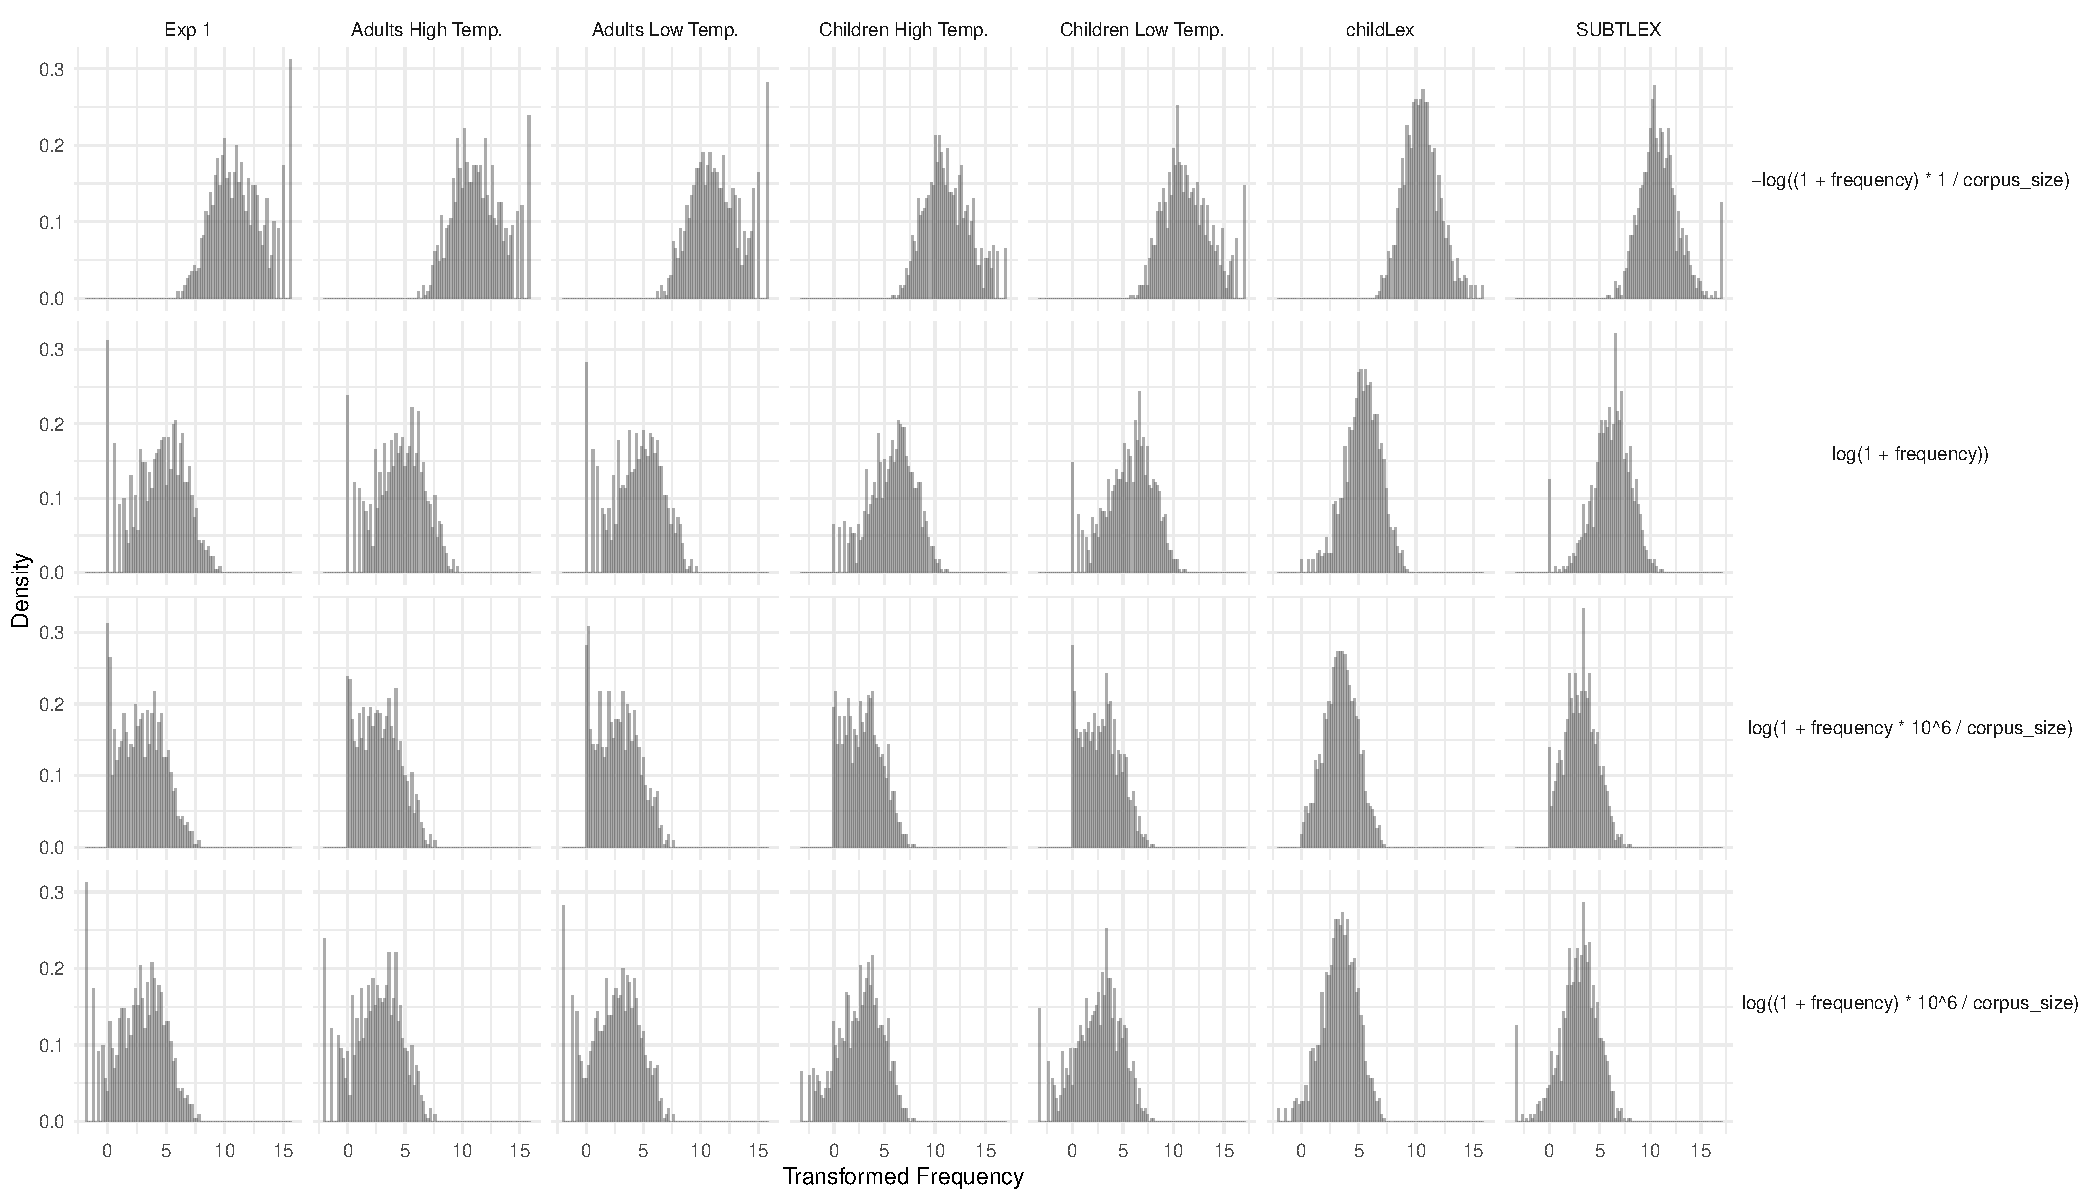
\includegraphics[width=\textwidth]{figures/histogram_plot_devel.pdf}}
    \caption{ Histograms of transformed word frequency values. The x-axis shows the transformed word frequency values, and the y-axis shows the density of the values. The facets show the different transformations and the different corpora. The transformation in the third row results in a hard cut-off at 0 while the other 3 transformations result in more normal-like distributions. }
    \label{fig:histogram_plot_devel}
  %\end{minipage}
\end{figure}

\clearpage

\begin{figure}[!htbp]
  %\centering
    \centering
    \begin{minipage}[t]{1\textwidth}
     \centering
    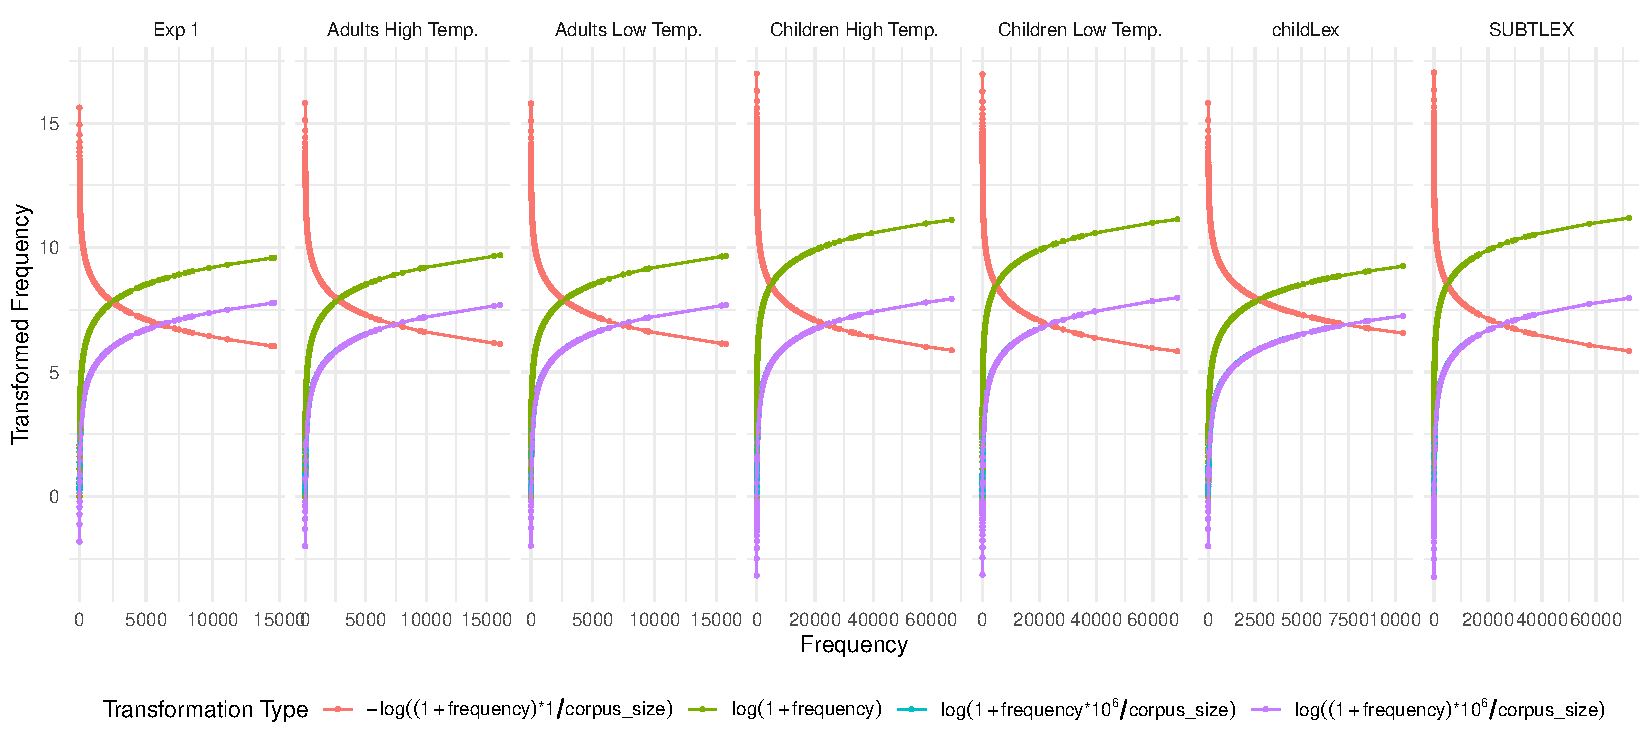
\includegraphics[width=\textwidth]{figures/scatter_plot2_devel.pdf}
    \caption{ Scatter plots of transformed word frequency values. The facets show the different corpora.}
    \label{fig:scatter_plot2_devel}

%   \end{minipage}
% \end{figure}

% % \vfill 

%   \begin{figure}[b]
%     \centering
%     \begin{minipage}[b]{1\textwidth}
  %\centering
    \centering
    %\begin{minipage}[t]{0.9\textwidth}
    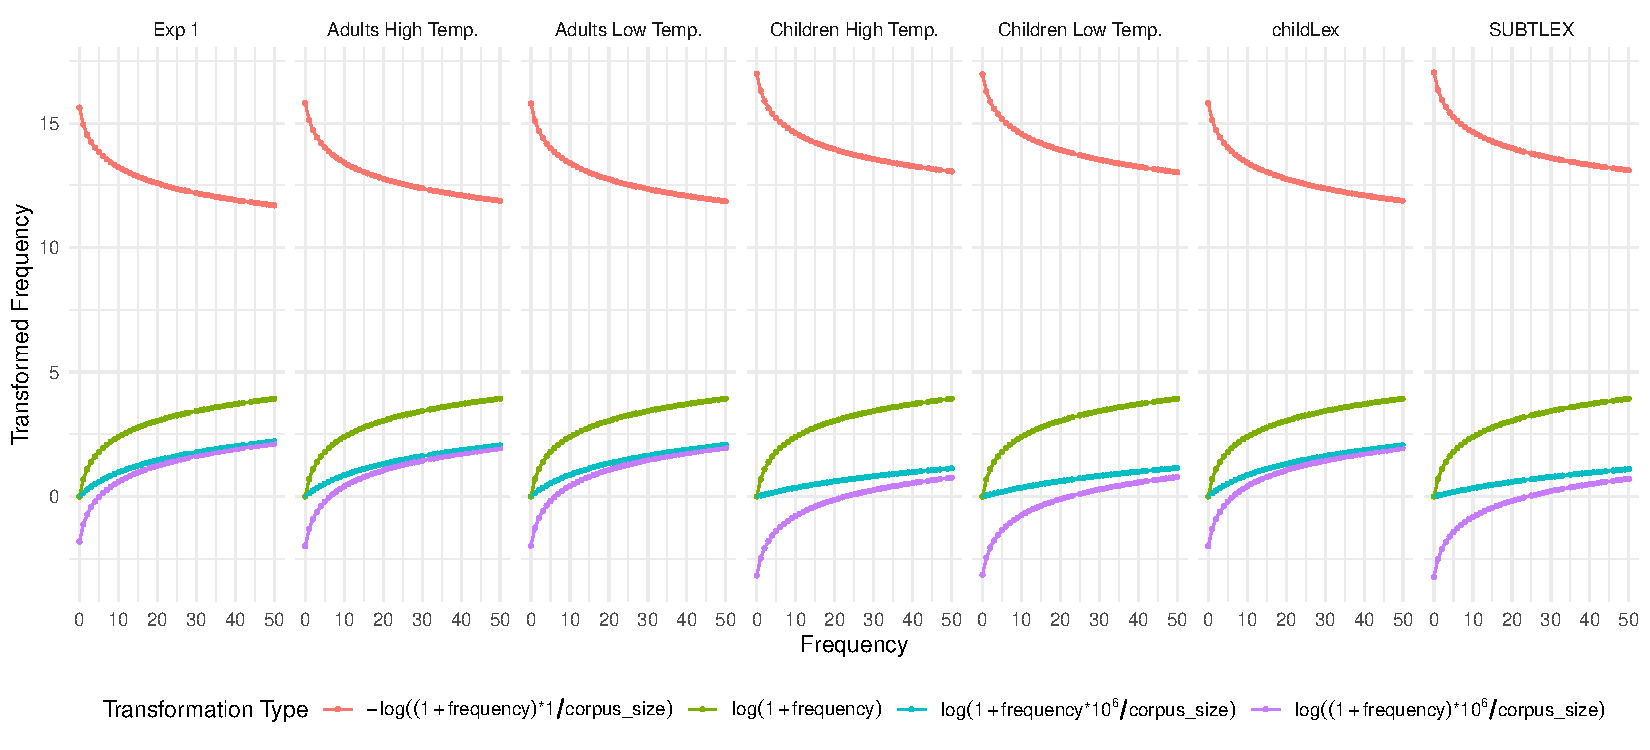
\includegraphics[width=\textwidth]{figures/scatter_plot_devel.pdf}
    \caption{ Zoomed in version of Figure \ref{fig:scatter_plot2_devel}, showing only observed word frequencies smaller than 50.}
    \label{fig:scatter_plot_devel}
  \end{minipage}
\end{figure}

\clearpage


\subsubsection{Correlation matrix}

Figure \ref{fig:cormat_devel} shows the correlation matrix for the subset of 1052 words from Devel \citep{schroter_developmental_2017}. 

\begin{figure}[!htbp]
  %\centering
  \centerline{
  %\begin{minipage}[t]{0.9\textwidth}
    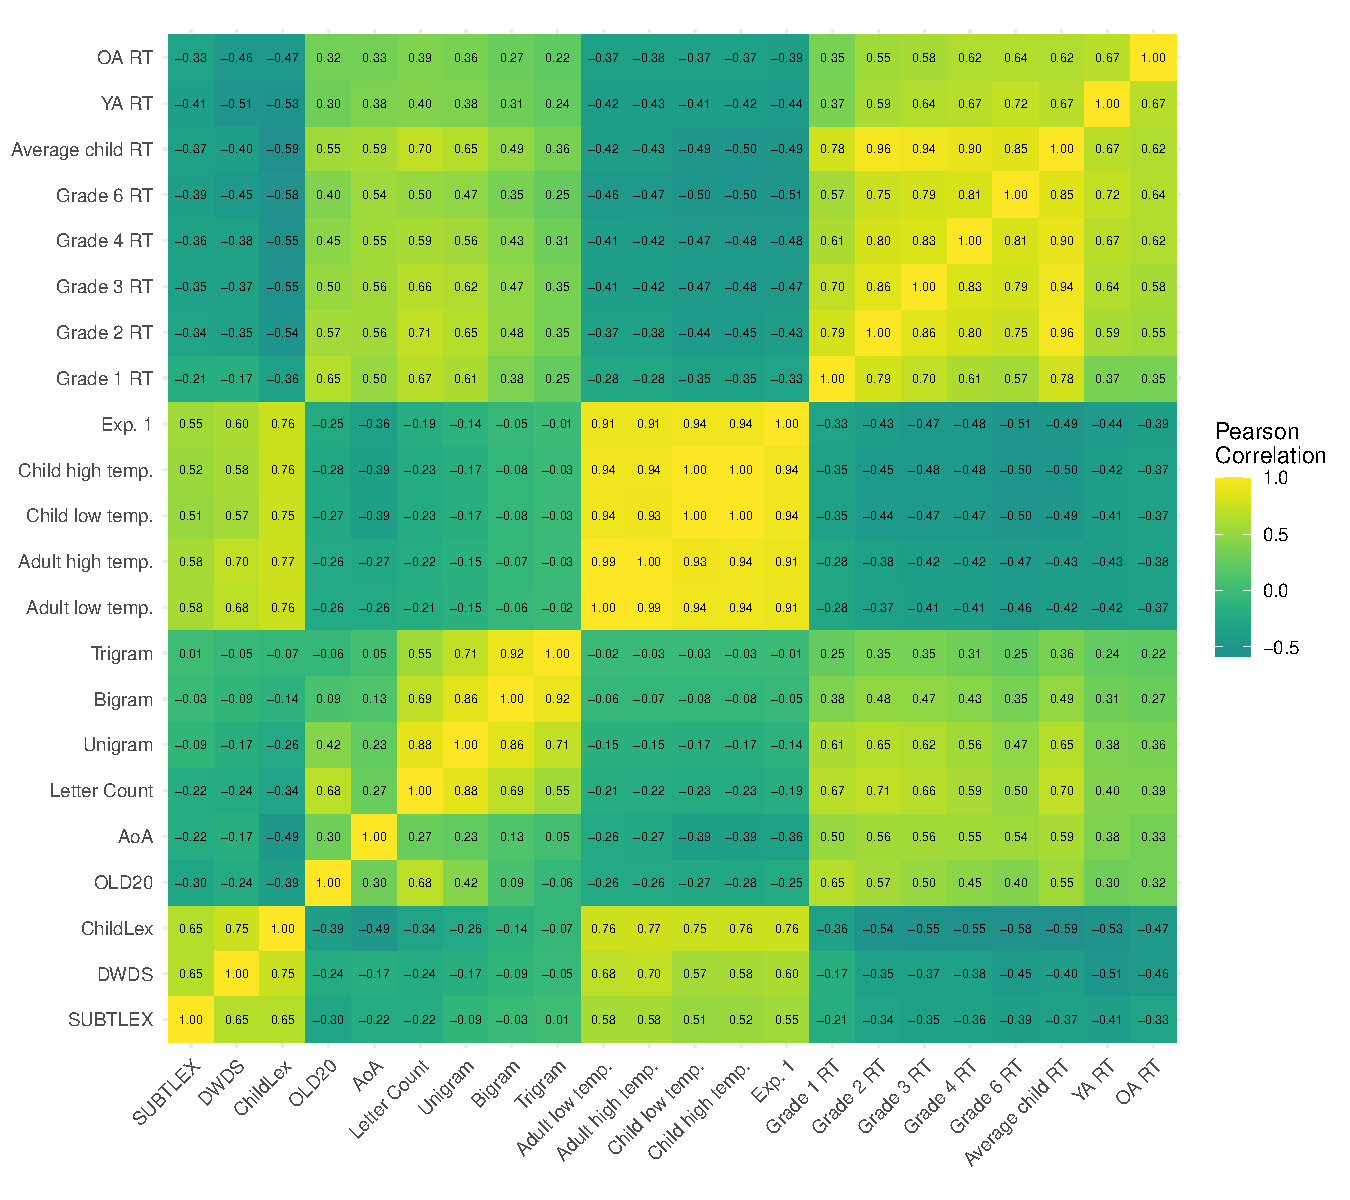
\includegraphics[width=\textwidth]{figures/correlation_matrix_devel.pdf}}
    \caption{Correlation matrix for the Devel subset of words for which Reaction times are available. The correlations with corpus-based word frequency measures are based on a $\log\left(\frac{(1 + \text{frequency}) \times 10^6}{\text{corpus\_size}}\right)$ transformation. These measures include: SUBTLEX, DWDS, childLex, adult low temp., adult high temp, children low temp., children high temp, and Exp. 1.}
    \label{fig:cormat_devel}
  %\end{minipage}
\end{figure}

\clearpage


\subsubsection{Words not in ChildLex or LLM corpus}

Tables \ref{words-adht}, \ref{words-adlt}, \ref{words-chht}, and \ref{words-chlt} show the top frequent words that occur in only one of both corpora, for all word lengths, and for words with more than 10 characters.

% latex table generated in R 4.2.2 by xtable 1.8-4 package
% Fri Jun 14 15:20:22 2024
\begin{table}[!htbp]
\caption{Words not in Childlex or in the AdLT corpus}
\centering
\begin{tabular}{llll}
  \hline
ChildLEX & ChildLEX $>$10 & GPT & GPT $>$10 \\ 
  \hline
daß & widersprach & Max & Charakteren \\ 
  1 & SternenClan & Anna & Schulvampire \\ 
  Wieso & Olchi-Kinder & Lena & einzustehen \\ 
  Gleich & kopfschüttelnd & Lisa & nahegelegenen \\ 
  guckte & vorwurfsvoll & Müller & thematisiert \\ 
  Bestimmt & Viertelstunde & Mia & unvergessliche \\ 
  mußte & augenblicklich & Emma & kindgerechte \\ 
  Jedenfalls & Mottenflügel & Paul & einfühlsame \\ 
  guckt & Anscheinend & – & Protagonisten \\ 
  kriegt & stirnrunzelnd & Harry & faszinierendes \\ 
   \hline
\end{tabular}
\label{words-adlt}
\end{table}

% latex table generated in R 4.2.2 by xtable 1.8-4 package
% Fri Jun 14 15:20:23 2024
\begin{table}[!htbp]
\caption{Words not in Childlex or in the AdHT corpus}
\centering
\begin{tabular}{llll}
  \hline
ChildLEX & ChildLEX $>$10 & GPT & GPT $>$10 \\ 
  \hline
daß & SternenClan & Max & Charakteren \\ 
  1 & Olchi-Kinder & Anna & nahegelegenen \\ 
  guckte & einigermaßen & Lena & einzustehen \\ 
  Bestimmt & Viertelstunde & – & unvergessliche \\ 
  Blattsee & Mottenflügel & Lisa & thematisiert \\ 
  mußte & stirnrunzelnd & Müller & Schulvampire \\ 
  Jedenfalls & Wolkenpfote & Mia & Protagonisten \\ 
  guckt & ausnahmsweise & Paul & kindgerechte \\ 
  kriegt & Ausgerechnet & Emma & herzerwärmende \\ 
  Dad & verschränkte & Julia & faszinierendes \\ 
   \hline
\end{tabular}
\label{words-adht}
\end{table}

% latex table generated in R 4.2.2 by xtable 1.8-4 package
% Fri Jun 14 15:20:23 2024
\begin{table}[!htbp]
\caption{Words not in Childlex or in the child high temperature corpus}
\centering
\begin{tabular}{llll}
  \hline
ChildLEX & ChildLEX $>$10 & GPT & GPT $>$10 \\ 
  \hline
wenigstens & Augenbrauen & Max & nahegelegenen \\ 
  hockte & SternenClan & Mia & Schulvampire \\ 
  Dem & unwillkürlich & Lina & unvergessliche \\ 
  Ihm & augenblicklich & Lena & Sternenfohlen \\ 
  Augenbrauen & Treppenhaus & Emma & einzustehen \\ 
  Immerhin & Einverstanden & Tim & Inselschüler \\ 
  nachher & Vorbeigehen & Felix & Schafgäääng \\ 
  Deswegen & Offensichtlich & Paul & KuchenMonster \\ 
  Außer & Krankenflügel & Lilli & SkaterBande \\ 
  SternenClan & irgendwelchen & Finn & abenteuerlustiger \\ 
   \hline
\end{tabular}
\label{words-chlt}
\end{table}

% latex table generated in R 4.2.2 by xtable 1.8-4 package
% Fri Jun 14 15:20:24 2024
\begin{table}[!htbp]
\caption{Words not in Childlex or in the child low temperature corpus}
\centering
\begin{tabular}{llll}
  \hline
ChildLEX & ChildLEX $>$10 & GPT & GPT $>$10 \\ 
  \hline
Neunauge & Anscheinend & Max & nahegelegenen \\ 
  Meinst & entgeistert & Mia & Schulvampire \\ 
  Madam & Mittlerweile & Lina & unvergessliche \\ 
  womöglich & verschränkte & Lena & Sternenfohlen \\ 
  Außer & Großmutters & Emma & Inselschüler \\ 
  gekriegt & gerunzelter & Tim & einzustehen \\ 
  Wozu & vorsichtshalber & Felix & Schafgäääng \\ 
  werd & umständlich & Paul & KuchenMonster \\ 
  Mich & Donnerwetter & Finn & SkaterBande \\ 
  Zumindest & unvermittelt & Anna & abenteuerlustiger \\ 
   \hline
\end{tabular}
\label{words-chht}
\end{table}

\clearpage

\subsubsection{Top frequency words occurring the least often in ChildLex or LLM corpus}

Tables \ref{words-adht-low}, \ref{words-adlt-low}, \ref{words-chht-low}, and \ref{words-chlt-low} show the top frequent words that occur the least often in the other corpus, for all word lengths, and for words with more than 10 characters.


% latex table generated in R 4.2.2 by xtable 1.8-4 package
% Fri Jun 14 15:20:22 2024
\begin{table}[!htbp]
\caption{The top frequent words that occur the least often in the other corpus, for all word lengths, and for words with more than 10 characters for the AdLT corpus}
\centering
\begin{tabular}{llll}
  \hline
ChildLEX & ChildLEX $>$10 & GPT & GPT $>$10 \\ 
  \hline
wenigstens & Hoffentlich & unterhaltsame & unterhaltsame \\ 
  Eigentlich & Schnupferich & lehrreiche & unschlagbares \\ 
  Hoffentlich & Zehenspitzen & Charaktere & Perspektiven \\ 
  vorhin & verächtlich & Bindung & Korallenschatz \\ 
  irgendwas & einigermaßen & Teamwork & vielfältige \\ 
  blöd & Pfannkuchen & unschlagbares & Sattelschlepper \\ 
  kreischte & entgeistert & humorvolle & unvergesslicher \\ 
  Mist & Ausgerechnet & Jack & weiterzuentwickeln \\ 
  Mehr & Mittlerweile & zeitlose & Mäusepension \\ 
  Bin & verschränkte & Überwinden & authentisch \\ 
   \hline
\end{tabular}
\label{words-adlt-low}
\end{table}

% latex table generated in R 4.2.2 by xtable 1.8-4 package
% Fri Jun 14 15:20:23 2024
\begin{table}[!htbp]
\caption{The top frequent words that occur the least often in the other corpus, for all word lengths, and for words with more than 10 characters for the AdHT corpus}
\centering
\begin{tabular}{llll}
  \hline
ChildLEX & ChildLEX $>$10 & GPT & GPT $>$10 \\ 
  \hline
jedenfalls & Wahrscheinlich & unterhaltsame & unterhaltsame \\ 
  Wahrscheinlich & Hoffentlich & Charaktere & unschlagbares \\ 
  flüstert & Unglaublich & lehrreiche & Perspektiven \\ 
  Hoffentlich & verständnislos & Bindung & vielfältige \\ 
  Quatsch & Premierminister & Teamwork & Mäusepension \\ 
  hockte & Seidenschnabel & humorvolle & Sattelschlepper \\ 
  Dem & Offensichtlich & unschlagbares & unzertrennliche \\ 
  Ihm & Erstklässler & zeitlose & Bedrohungen \\ 
  Meinst & Großmutters & Ermittler & vielschichtigen \\ 
  gucken & irgendwelchen & Poppins & Korallenschatz \\ 
   \hline
\end{tabular}
\label{words-adht-low}
\end{table}

% latex table generated in R 4.2.2 by xtable 1.8-4 package
% Fri Jun 14 15:20:23 2024
\begin{table}[!htbp]
\caption{The top frequent words that occur the least often in the other corpus, for all word lengths, and for words with more than 10 characters for the child high temperature corpus}
\centering
\begin{tabular}{llll}
  \hline
ChildLEX & ChildLEX $>$10 & GPT & GPT $>$10 \\ 
  \hline
wenigstens & Augenbrauen & unschlagbares & unschlagbares \\ 
  hockte & SternenClan & Brumm & unzertrennliche \\ 
  Dem & unwillkürlich & unzertrennliche & Sattelschlepper \\ 
  Ihm & augenblicklich & Sattelschlepper & unvergessliches \\ 
  Augenbrauen & Treppenhaus & unvergessliches & aufgewecktes \\ 
  Immerhin & Einverstanden & Charaktere & Mäusepension \\ 
  nachher & Vorbeigehen & Poppins & unvergesslicher \\ 
  Deswegen & Offensichtlich & Holle & Korallenschatz \\ 
  Außer & Krankenflügel & aufgewecktes & Schulgespenst \\ 
  SternenClan & irgendwelchen & Zaubermaus & unterhaltsame \\ 
   \hline
\end{tabular}
\label{words-chlt-low}
\end{table}

% latex table generated in R 4.2.2 by xtable 1.8-4 package
% Fri Jun 14 15:20:24 2024
\begin{table}[!htbp]
\caption{The top frequent words that occur the least often in the other corpus, for all word lengths, and for words with more than 10 characters for the child low temperature corpus}

\centering
\begin{tabular}{llll}
  \hline
ChildLEX & ChildLEX $>$10 & GPT & GPT $>$10 \\ 
  \hline
Neunauge & Anscheinend & unschlagbares & unschlagbares \\ 
  Meinst & entgeistert & Brumm & unzertrennliche \\ 
  Madam & Mittlerweile & unzertrennliche & unvergessliches \\ 
  womöglich & verschränkte & Charaktere & Sattelschlepper \\ 
  Außer & Großmutters & Poppins & aufgewecktes \\ 
  gekriegt & gerunzelter & unvergessliches & unvergesslicher \\ 
  Wozu & vorsichtshalber & Sattelschlepper & Schulgespenst \\ 
  werd & umständlich & Holle & Mäusepension \\ 
  Mich & Donnerwetter & Bindung & Korallenschatz \\ 
  Zumindest & unvermittelt & aufgewecktes & unterhaltsame \\ 
   \hline
\end{tabular}
\label{words-chht-low}
\end{table}

\clearpage





\end{document}
